
% Page margins, header and footer positions
\usepackage{geometry}
\geometry{
    a4paper,
    total={210mm,297mm},
    left=25mm,
    right=25mm,
    top=30mm,
    bottom=25mm,
    headsep=7mm
}

\interfootnotelinepenalty=10000

%To display filling dots in the TOC for all entries
\usepackage[titles]{tocloft}
\renewcommand{\cftsecleader}{\cftdotfill{\cftdotsep}}


%PACKAGES
\usepackage{wasysym}
\usepackage{pifont}

\newcommand{\supported}{\ding{52}\xspace}
\newcommand{\unsupported}{\ding{55}\xspace}
\newcommand{\partsupported}{\textcolor{black!40}{\ding{52}}\xspace}
\newcommand{\lowsupported}{\textcolor{black!20}{\ding{52}}\xspace}
\newcommand{\unknowsupported}{\textbf{?}\xspace}

%Font: Times
\usepackage{times}
%Change monospaced font
\renewcommand{\ttdefault}{lmtt}

%tables
\usepackage{tabu}
\usepackage{tabularx}
\usepackage{ltablex}
\usepackage{longtable}
\usepackage{float} % To allow the use of H modifier in long tables

%landscape mode
\usepackage{pdflscape}
\usepackage{rotating}
\usepackage{caption}

%make landscape mode be sensitive to even and odd pages
%start
\def\myrotate{\ifodd\c@page\else-\fi 90}
\makeatletter
\global\let\orig@begin@landscape=\landscape%
\global\let\orig@end@landscape=\endlandscape%
\gdef\@true{1}
\gdef\@false{0}
\gdef\landscape{%
    \global\let\within@landscape=\@true%
    \orig@begin@landscape%
}%
\gdef\endlandscape{%
    \orig@end@landscape%
    \global\let\within@landscape=\@false%
}%
\@ifpackageloaded{pdflscape}{%
    \gdef\pdf@landscape@rotate{\PLS@Rotate}%
}{
    \gdef\pdf@landscape@rotate#1{}%
}
\let\latex@outputpage\@outputpage
\def\@outputpage{
    \ifx\within@landscape\@true%
        \if@twoside%
            \ifodd\c@page%
                \gdef\LS@rot{\setbox\@outputbox\vbox{%
                    \pdf@landscape@rotate{-90}%
                    \hbox{\rotatebox{90}{\hbox{\rotatebox{180}{\box\@outputbox}}}}}%
                }%
            \else%
                \gdef\LS@rot{\setbox\@outputbox\vbox{%
                    \pdf@landscape@rotate{+90}%
                    \hbox{\rotatebox{90}{\hbox{\rotatebox{0}{\box\@outputbox}}}}}%
                }%
            \fi%
        \else%
            \gdef\LS@rot{\setbox\@outputbox\vbox{%
                \pdf@landscape@rotate{+90}%
                \hbox{\rotatebox{90}{\hbox{\rotatebox{0}{\box\@outputbox}}}}}%
            }%
        \fi%
    \fi%
    \latex@outputpage%
}
\makeatother
%end
%graphics
\usepackage{graphicx}
\usepackage[dvipsnames, table]{xcolor}
%If you upload images from PC, you need to insert code for the path here (different for Windows and Unix OS)

%References
%\usepackage{xpatch}
%\usepackage[backend=biber, style=numeric, citestyle=numeric, sorting=none]{biblatex}
%\addbibresource{main.bib}

%Other
\usepackage{ifthen}
\usepackage{xspace}
\usepackage{enumitem}
\usepackage{amssymb}
\usepackage[pdftex, colorlinks]{hyperref}
\newcommand{\comment}[1]{{\color{Red}$\blacktriangleright$ Comment: #1 $\blacktriangleleft$}}
% Some utilities\ldots
\usepackage{soul}
\usepackage{tikz}

\usetikzlibrary{calc}
\usetikzlibrary{decorations.pathmorphing}


\makeatletter

\newcommand{\defhighlighter}[3][]{%
  \tikzset{every highlighter/.style={color=#2, fill opacity=#3, #1}}%
}

\defhighlighter{yellow}{.5}

\newcommand{\highlight@DoHighlight}{
  \fill [ decoration = {random steps, amplitude=1pt, segment length=15pt}
        , outer sep = -15pt, inner sep = 0pt, decorate
       , every highlighter, this highlighter ]
        ($(begin highlight)+(0,8pt)$) rectangle ($(end highlight)+(0,-3pt)$) ;
}

\newcommand{\highlight@BeginHighlight}{
  \coordinate (begin highlight) at (0,0) ;
}

\newcommand{\highlight@EndHighlight}{
  \coordinate (end highlight) at (0,0) ;
}

\newdimen\highlight@previous
\newdimen\highlight@current

\DeclareRobustCommand*\highlight[1][]{%
  \tikzset{this highlighter/.style={#1}}%
  \SOUL@setup
  %
  \def\SOUL@preamble{%
    \begin{tikzpicture}[overlay, remember picture]
      \highlight@BeginHighlight
      \highlight@EndHighlight
    \end{tikzpicture}%
  }%
  %
  \def\SOUL@postamble{%
    \begin{tikzpicture}[overlay, remember picture]
      \highlight@EndHighlight
      \highlight@DoHighlight
    \end{tikzpicture}%
  }%
  %
  \def\SOUL@everyhyphen{%
    \discretionary{%
      \SOUL@setkern\SOUL@hyphkern
      \SOUL@sethyphenchar
      \tikz[overlay, remember picture] \highlight@EndHighlight ;%
    }{%
    }{%
      \SOUL@setkern\SOUL@charkern
    }%
  }%
  %
  \def\SOUL@everyexhyphen##1{%
    \SOUL@setkern\SOUL@hyphkern
    \hbox{##1}%
    \discretionary{%
      \tikz[overlay, remember picture] \highlight@EndHighlight ;%
    }{%
    }{%
      \SOUL@setkern\SOUL@charkern
    }%
  }%
  %
  \def\SOUL@everysyllable{%
    \begin{tikzpicture}[overlay, remember picture]
      \path let \p0 = (begin highlight), \p1 = (0,0) in \pgfextra
        \global\highlight@previous=\y0
        \global\highlight@current =\y1
      \endpgfextra (0,0) ;
      \ifdim\highlight@current < \highlight@previous
        \highlight@DoHighlight
        \highlight@BeginHighlight
      \fi
    \end{tikzpicture}%
    \the\SOUL@syllable
    \tikz[overlay, remember picture] \highlight@EndHighlight ;%
  }%
  \SOUL@
}

\makeatother

% Common abbrev. are set as commands to ensure proper spacing after the dot
\RequirePackage{xspace}
\newcommand{\ie}{i.e.\@\xspace}
\newcommand{\aka}{a.k.a.\@\xspace}
\newcommand{\Ie}{I.e.\@\xspace}
\newcommand{\cf}{cf.\@\xspace}
\newcommand{\Cf}{Cf.\@\xspace}
\newcommand{\eg}{e.g.\@\xspace}
\newcommand{\Eg}{E.g.\@\xspace}
\newcommand{\etal}{et al.\@\xspace}
\newcommand{\etc}{etc.\@\xspace}
\newcommand{\wrt}{w.r.t.\@\xspace}
\newcommand{\Wrt}{W.r.t.\@\xspace}



\date{}


\documentclass[11pt,twoside]{article}
\usepackage[utf8]{inputenc}
\usepackage[T1]{fontenc}

% Page margins, header and footer positions
\usepackage{geometry}
\geometry{
 a4paper,
 total={210mm,297mm},
 left=25mm,
 right=25mm,
 top=30mm,
 bottom=25mm,
 headsep=7mm
}

\interfootnotelinepenalty=10000

% To display filling dots in the TOC for all entries
\usepackage[titles]{tocloft}
\renewcommand{\cftsecleader}{\cftdotfill{\cftdotsep}}

% Graphics
\usepackage{graphicx}
\usepackage[dvipsnames, table]{xcolor}

% Define new header and footer style
\usepackage{fancyhdr}

\pagestyle{fancy}
\fancyhf{}
\lhead{\color{Gray}{\small{SE2 - project by Emanuele Cimino, Gabriele Lorenzetti}}}
\lfoot{\textcolor{Gray}{\small{Copyright © 2024, Emanuele Cimino - Gabriele Lorenzetti – All rights reserved}}}
\rfoot{\textcolor{Gray}{\thepage}}
\renewcommand{\headrulewidth}{0pt}

% PACKAGES
\usepackage{wasysym}
\usepackage{pifont}

\newcommand{\supported}{\ding{52}\xspace}
\newcommand{\unsupported}{\ding{55}\xspace}
\newcommand{\partsupported}{\textcolor{black!40}{\ding{52}}\xspace}
\newcommand{\lowsupported}{\textcolor{black!20}{\ding{52}}\xspace}
\newcommand{\unknowsupported}{\textbf{?}\xspace}

% Font: Times
\usepackage{times}
% Change monospaced font
\renewcommand{\ttdefault}{lmtt}

% Tables
\usepackage{tabu}
\usepackage{tabularx}
\usepackage{ltablex}
\usepackage{longtable}
\usepackage{float}

% Landscape mode
\usepackage{pdflscape}
\usepackage{rotating}
\usepackage{caption}

% Make landscape mode be sensitive to even and odd pages
\def\myrotate{\ifodd\c@page\else-\fi 90}
\makeatletter
\global\let\orig@begin@landscape=\landscape%
\global\let\orig@end@landscape=\endlandscape%
\gdef\@true{1}
\gdef\@false{0}
\gdef\landscape{%
    \global\let\within@landscape=\@true%
    \orig@begin@landscape%
}%
\gdef\endlandscape{%
    \orig@end@landscape%
    \global\let\within@landscape=\@false%
}%
\@ifpackageloaded{pdflscape}{%
    \gdef\pdf@landscape@rotate{\PLS@Rotate}%
}{
    \gdef\pdf@landscape@rotate#1{}%
}
\let\latex@outputpage\@outputpage
\def\@outputpage{
    \ifx\within@landscape\@true%
        \if@twoside%
            \ifodd\c@page%
                \gdef\LS@rot{\setbox\@outputbox\vbox{%
                    \pdf@landscape@rotate{-90}%
                    \hbox{\rotatebox{90}{\hbox{\rotatebox{180}{\box\@outputbox}}}}}%
                }%
            \else%
                \gdef\LS@rot{\setbox\@outputbox\vbox{%
                    \pdf@landscape@rotate{+90}%
                    \hbox{\rotatebox{90}{\hbox{\rotatebox{0}{\box\@outputbox}}}}}%
                }%
            \fi%
        \else%
            \gdef\LS@rot{\setbox\@outputbox\vbox{%
                \pdf@landscape@rotate{+90}%
                \hbox{\rotatebox{90}{\hbox{\rotatebox{0}{\box\@outputbox}}}}}%
            }%
        \fi%
    \fi%
    \latex@outputpage%
}
\makeatother



% Other
\usepackage{ifthen}
\usepackage{xspace}
\usepackage{enumitem}
\usepackage{amssymb}
\usepackage[pdftex, colorlinks]{hyperref}
\newcommand{\comment}[1]{{\color{Red}$\blacktriangleright$ Comment: #1 $\blacktriangleleft$}}

% Some utilities
\usepackage{soul}
\usepackage{tikz}

\usetikzlibrary{calc}
\usetikzlibrary{decorations.pathmorphing}


\makeatletter

\newcommand{\defhighlighter}[3][]{%
  \tikzset{every highlighter/.style={color=#2, fill opacity=#3, #1}}%
}

\defhighlighter{yellow}{.5}

\newcommand{\highlight@DoHighlight}{
  \fill [ decoration = {random steps, amplitude=1pt, segment length=15pt}
        , outer sep = -15pt, inner sep = 0pt, decorate
       , every highlighter, this highlighter ]
        ($(begin highlight)+(0,8pt)$) rectangle ($(end highlight)+(0,-3pt)$) ;
}

\newcommand{\highlight@BeginHighlight}{
  \coordinate (begin highlight) at (0,0) ;
}

\newcommand{\highlight@EndHighlight}{
  \coordinate (end highlight) at (0,0) ;
}

\newdimen\highlight@previous
\newdimen\highlight@current

\DeclareRobustCommand*\highlight[1][]{%
  \tikzset{this highlighter/.style={#1}}%
  \SOUL@setup
  %
  \def\SOUL@preamble{%
    \begin{tikzpicture}[overlay, remember picture]
      \highlight@BeginHighlight
      \highlight@EndHighlight
    \end{tikzpicture}%
  }%
  %
  \def\SOUL@postamble{%
    \begin{tikzpicture}[overlay, remember picture]
      \highlight@EndHighlight
      \highlight@DoHighlight
    \end{tikzpicture}%
  }%
  %
  \def\SOUL@everyhyphen{%
    \discretionary{%
      \SOUL@setkern\SOUL@hyphkern
      \SOUL@sethyphenchar
      \tikz[overlay, remember picture] \highlight@EndHighlight ;%
    }{%
    }{%
      \SOUL@setkern\SOUL@charkern
    }%
  }%
  %
  \def\SOUL@everyexhyphen##1{%
    \SOUL@setkern\SOUL@hyphkern
    \hbox{##1}%
    \discretionary{%
      \tikz[overlay, remember picture] \highlight@EndHighlight ;%
    }{%
    }{%
      \SOUL@setkern\SOUL@charkern
    }%
  }%
  %
  \def\SOUL@everysyllable{%
    \begin{tikzpicture}[overlay, remember picture]
      \path let \p0 = (begin highlight), \p1 = (0,0) in \pgfextra
        \global\highlight@previous=\y0
        \global\highlight@current =\y1
      \endpgfextra (0,0) ;
      \ifdim\highlight@current < \highlight@previous
        \highlight@DoHighlight
        \highlight@BeginHighlight
      \fi
    \end{tikzpicture}%
    \the\SOUL@syllable
    \tikz[overlay, remember picture] \highlight@EndHighlight ;%
  }%
  \SOUL@
}

\makeatother

% Common abbrev. are set as commands to ensure proper spacing after the dot
\RequirePackage{xspace}
\newcommand{\ie}{i.e.\@\xspace}
\newcommand{\aka}{a.k.a.\@\xspace}
\newcommand{\Ie}{I.e.\@\xspace}
\newcommand{\cf}{cf.\@\xspace}
\newcommand{\Cf}{Cf.\@\xspace}
\newcommand{\eg}{e.g.\@\xspace}
\newcommand{\Eg}{E.g.\@\xspace}
\newcommand{\etal}{et al.\@\xspace}
\newcommand{\etc}{etc.\@\xspace}
\newcommand{\wrt}{w.r.t.\@\xspace}
\newcommand{\Wrt}{W.r.t.\@\xspace}

\begin{document}

% TITLE PAGE
\begin{titlepage}
% LOGO
{\begin{table}[t!]
\centering
\begin{tabu} to \textwidth { X[1.3,r,p] X[1.7,l,p] }
\textcolor{Black}
{\textbf{\small{Software engineering 2 project -  Lorenzetti Cimino}}} & 
\includegraphics[scale=0.5]{Images/PolimiLogo}
\end{tabu}
\end{table}}~\\ [7cm]

% TITLE 
\begin{flushleft}
{\textcolor{Black}{\textbf{\Huge{Requirement Analysis and Specification
        Document}}}} \\ [1cm]
\end{flushleft}
\end{titlepage}

% Define deliverable specific info
\begin{table}[h!]
\begin{tabu} to \textwidth { X[0.3,r,p] X[0.7,l,p] }
\hline
\textbf{Deliverable:} & RASD\\
\textbf{Title:} & Requirement Analysis and Verification Document \\
\textbf{Authors:} & Gabriele Lorenzetti-Emanuele Cimino \\
\textbf{Version:} & 1.0 \\ 
\textbf{Date:} & 22-december-2024 \\
\textbf{Download page:} & LINK TO YOUR REPOSITORY \\
\textbf{Copyright:} & Copyright © 2024, Gabriele Lorenzetti-Emanuele Cimino – All rights reserved \\
\hline
\end{tabu}
\end{table}

\setcounter{page}{2}

\newpage
\addcontentsline{toc}{section}{Table of Contents}
\tableofcontents
\newpage
\addcontentsline{toc}{section}{List of Figures}
\listoffigures
\addcontentsline{toc}{section}{List of Tables}
\listoftables

\clearpage
{\color{Black}{\section{Introduction}}}
\label{sect:Introduction}
\subsection{Purpose}
If you are looking for an internship or want to offer one, you are in the right place, S\&C will help you!\\
Student\&Companies is a platform that helps match university students looking for internships and companies offering them.\\
The primary objective of the platform are as follow:
\begin{itemize}
    \item Students can search for an internship on their own or can be informed when an internship request compatible with their CV and characteristics is published.
    \item The system will help both student and companies find each other, by a system called "recommendation" that helps find the correspondence between the characteristic offered by the student and the ones asked by the company.
    \item The management of the selection process. 
    \item The monitoring of the execution of the internships, including statistics, feedback, and complaints.
\end{itemize}
\subsubsection{Goals}
\textbf{[G1]:} All unregistered students and companies must be able to subscribe and login to the S\&C platform.\\
\textbf{[G2]:} Students and companies must be able to write their descriptions and preferences.\\
\textbf{[G3]:} Students must be able to complete their CV.\\
\textbf{[G4]:} Companies must be able to create internship offers.\\
\textbf{[G5]:} Students must be able to search for an internship.\\
\textbf{[G6]:} Student and Company are informed when there is a match between them.\\
\textbf{[G7]:} Monitoring of the execution of the internships.\\
\textbf{[G8]:} Statistics collection.\\
\textbf{[G9]:} Feedbacks collection.\\
\textbf{[G10]:} Companies rank based on feedback. 
\subsection{Scope}
S\&C allows student and companies to communicate easily in a guided environment.\\
Students are able to upload their CVs and express their preferences about the work environment.\\
Companies upload their internship offers through the platform.\\
Students need to be able to actively search for an internship, through a keyword or by selecting some preferences.\\
The system  implements a process called "recommendation": it's a mechanisms that apply a research through the internship preferences and students characteristics, to inform students when an interesting internship becomes available and informs also companies that a student matches with theirs preferences.\\
The platform also propose to help companies in the selection process. When there is a match between the two parts, and both of them accept it, the process start. Companies feed questionnaire to the students and collect their responses to evaluate their fit with the company and can finalize the selection. 
The platform also stores statistics about internship that are offered by companies and the feedback from the students.
\subsubsection{Phenomena}
\begin{table}[H]
\renewcommand\arraystretch{1.5}
    \centering
    \begin{tabular}{|ccc|}
        \hline
        \rowcolor{BurntOrange}
        \textbf{Phenomenon}&  \textbf{Who controls it?}& \textbf{Is shared?}\\
        \hline
        Users decides to use S\&C&  W& N\\
        \hline
        User registration&  W& Y\\
        \hline
        User login& W& Y\\
        \hline
        Check username and password&  M& N\\
        \hline
        Student create CV&  W& Y\\
        \hline
        Company create offer&  W& Y\\
        \hline
        Recommendation process start& M& N\\
        \hline
        Student search offer&  W& Y\\
        \hline
        Match notification&  M& Y\\
        \hline
        Match acceptation&  W& Y\\
        \hline
        Student's feedback&  W& Y\\
        \hline
        Statistics collection&  M& N\\
        \hline
        Companies rank computation&  M& N\\
        \hline
        Companies rank publication&  M& Y\\
        \hline
        Interview process start&  M& N\\
        \hline
        Form sending&  M& Y\\
        \hline
        Form compilation&  W& Y\\
        \hline
        Interview schedule&  M& Y\\
        \hline
    \end{tabular}
    \caption{Phenomena}
    \label{Phenomena}
\end{table}
\subsection{Definitions, Acronyms, Abbreviations}
\subsubsection{Definitions}
\subsubsection{Acronyms}
\begin{itemize}
    \item \textbf{S\&C:} Student and Companies
    \item \textbf{CV:} curriculum vitae
    \item \textbf{Zoom:} Zoom platform
    \item \textbf{G:} goal
    \item \textbf{A:} assumption
    \item \textbf{UC:} use cases
    \item \textbf{AD:} activity diagram
\end{itemize}
\subsubsection{Abbreviations}
\subsection{Revision history}
\subsection{Reference Documents}
\begin{itemize}
    \item Slides of the course “Software Engineering 2”.
    \item Michael Jackson, The World and the Machine.
    \item Specification document "01. Assignment RDD AY 2024-2025”
    \item Alloy documentation - https://alloytools.org/documentation.html
\end{itemize}
\subsection{Document Structure}
\begin{enumerate}
    \item \textbf{Introduction:} a description of the problem showing the purpose and the scope of the application. In order to precisely delineate the scope, phenomena and goals related to the problem are identified. In this section information about terms used in this document is also present, along with references and revision history.
    \item \textbf{Overall Descriptions:} a high-level view of the project. The perspective of the product is developed with scenarios and descriptions about requirements of the service interfaces. Product functions describe the required functions of the system in order to fulfill the goals as specified by the stakeholders. Furthermore, possible actors are also identified in the user user characteristics section. In the end there is a list of the taken domain assumptions.
    \item \textbf{Specific Requirements:} detailed description of the user interface, function and non-functional service requirements specification. Functional Requirements are supported from specific use cases and mappings that permit to acknowledge how the goals are satisfied.
    \item \textbf{Formal Analysis Using Alloy:} Alloy model useful in checking necessary properties of the system, and generating possible world in which the same will operate.
    \item \textbf{Effort Spent:} hours spent by each group member on the various activities related to the document developing.
\end{enumerate}
%what you write here is a comment that is not shown in the final text

\clearpage
{\color{Black}{\section{Overall Description}}}
\label{sect:Overall Description}
\subsection{Product perspective}

\subsubsection{Scenarios}
Here are presented possible scenarios for the users of the S\&C platform.
\begin{enumerate}
    \item \textbf{A company wants to have access to the S\&C services:}\\
    A company would like to offer one or more internships to students, but does not know how to find/contact them and how to choose the most suitable one. Therefore, the company registers on the S\&C platform, entering its name, an email address, a password, its VAT number, contacts, a description of themselves and what it is interested in within relative fields. For subsequent times, to access it only has his/her e-mail and password.
    \item \textbf{A student wants to have access to the S\&C services:}\\
    A student wants to have the opportunity to gain more experience during his/her studies or, also, to earn some money during his/her studies and he/she doesn't know which company to choose, so he/she subscribes to the platform S\&C. When subscribing, the student enters his/her first name, last name, e-mail, a password, contacts, a description of itself and the answers to questions about his/her preferences so as to facilitate the recommendation system, within relative fields. For subsequent times, to access he/she only has to enter his/her e-mail and password.
    \item \textbf{A company insert internship offers, changes its personal data and description}\\
    Now that it is inside the platform, the company can add its new internship offer, inserting the title, an adequate description, the characteristics and the questions to be included in the relative form that will be filled out by the student at the beginning of the selection process. Or it can modify/update existing offers, its personal data and descriptions.
    \item \textbf{A student insert his/her CV, changes his/her personal data, descriptions and preferences}\\
    Now that it is inside the platform the student can insert or modify his/her CV by uploading it as a PDF. He/She can also modify/update his/her personal data and description.
    \item \textbf{A student search for an internship}\\
    To search for an internship, the student must enter a keyword or the name of a company in the search bar, and can customize his/her search through filters. Once he/she has chosen the offer that is right for him/her, he/she can request to start the selection process and S\&C will take care of notifying the company in question.
    \item \textbf{Recommendation system notification}\\
    Based on the preference inserted by the student and the companies and the statistical analysis from the data collected by the platform, they get notified when a match is available, throughout the research made by the recommendation system.
    \item \textbf{Acceptance phase}\\
    When the student or the company receive a notification, they have to accept or refuse it through a button. if they accept they must indicate their availability spots and the platform will find the first free spot in common for the video interview. If that does not exists notify both with their e-mail.
    \item \textbf{Selection process}\\
    After the establishment of a contact, the selection process start, and the student has to compile a form with specific questions to check if he/she really fit with the position. Then they proceed with the scheduled interview through a Zoom link provided by the platform. After the interview, both participant can accept or not the collaboration.
    \item \textbf{Ending internship}\\
    At the end of the internship the student and the company can leave feedback on the counterpart.    
\end{enumerate}

\subsubsection{Domain-level Diagram}
\begin{figure}[H]
    \centering
    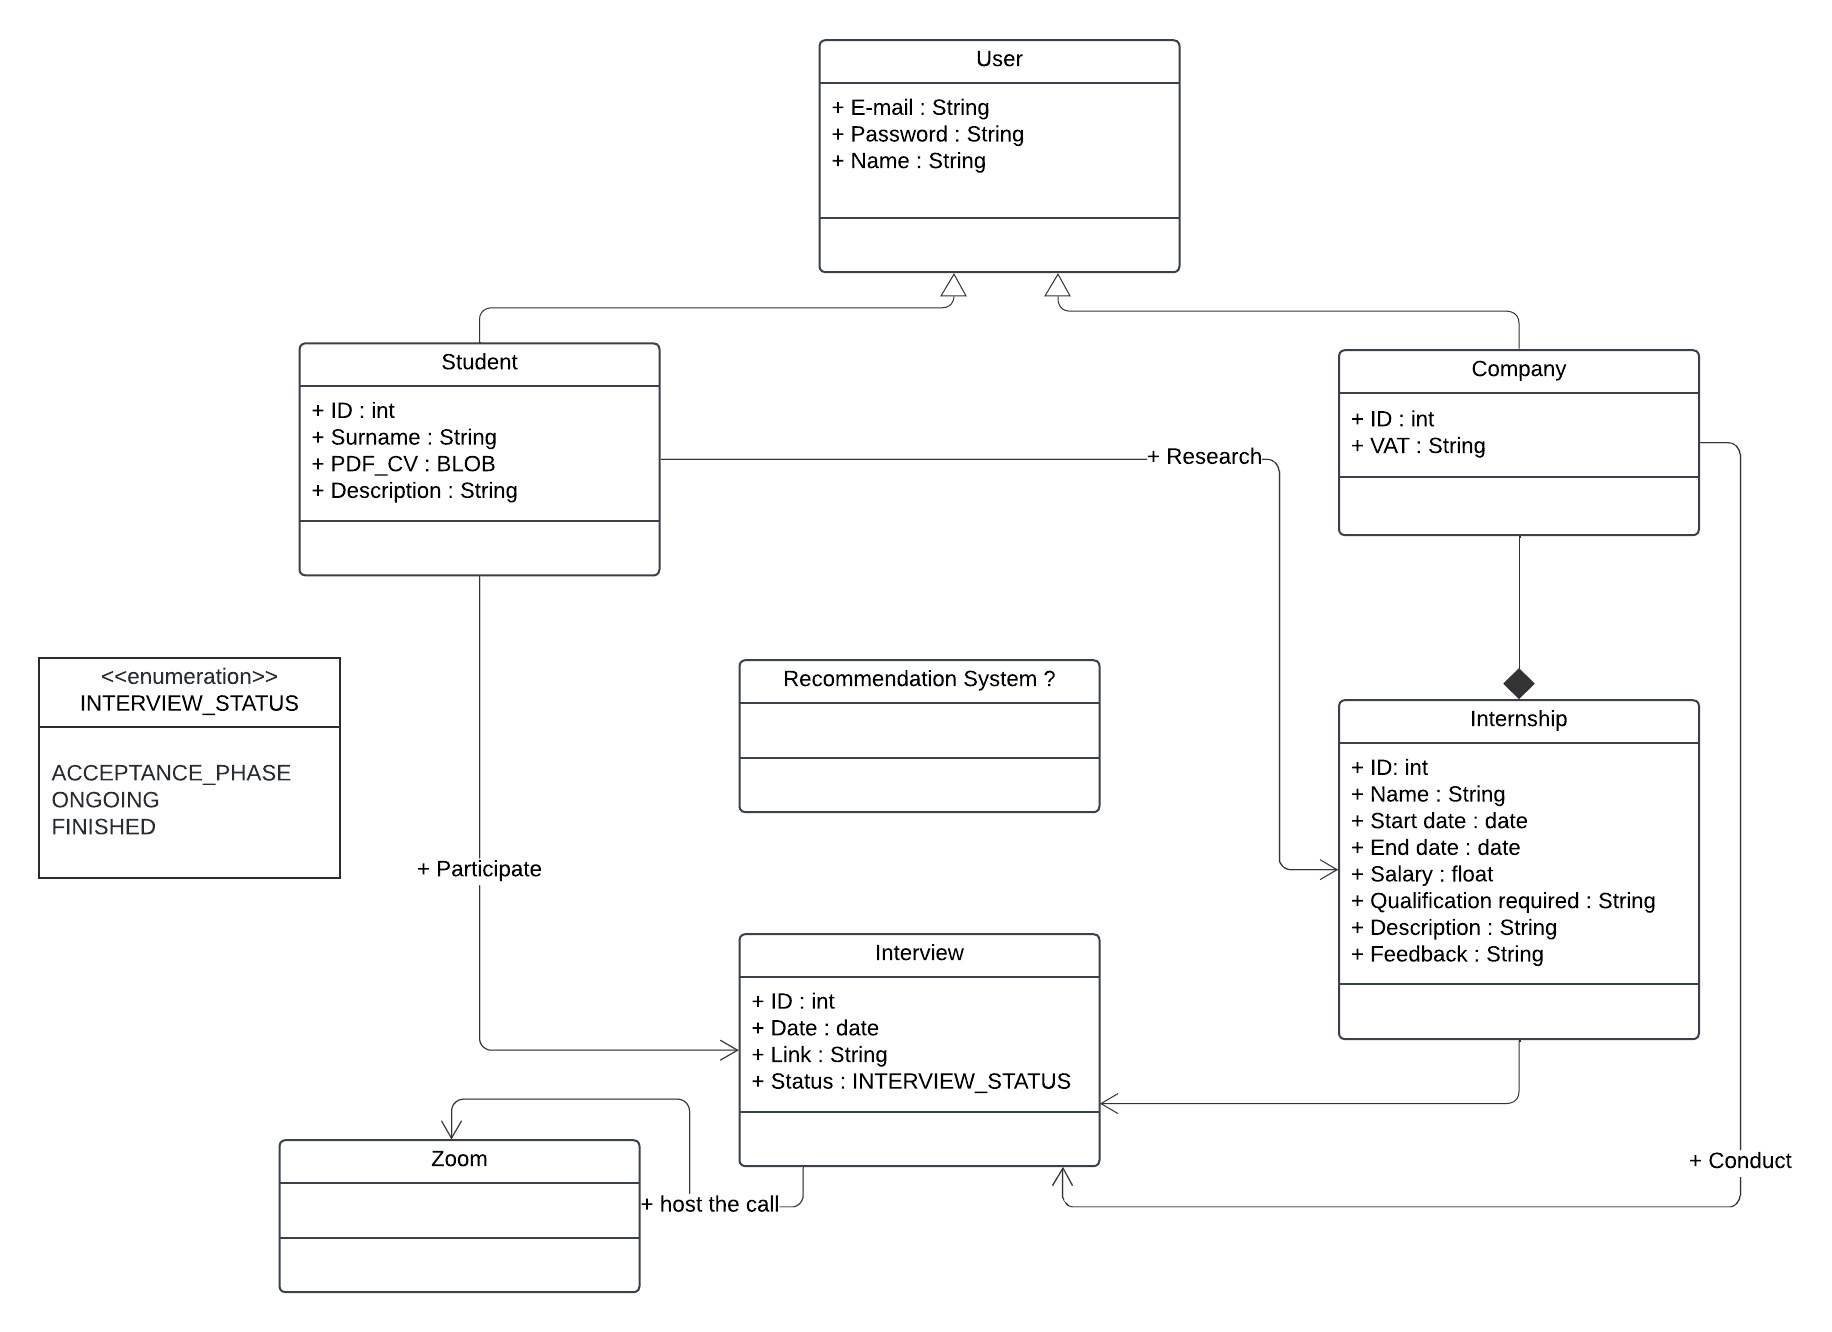
\includegraphics[width=\textwidth]{Images/Class diagram.png}
    \caption{Class diagram}
    \label{Class diagram}
\end{figure}

\subsubsection{State Diagrams}
State diagrams describe the behavior of the system while considering all possible states the system can deal with when an event occurs. This analysis helps to clarify the most critical aspects of the system.
\begin{figure}[H]
    \centering
    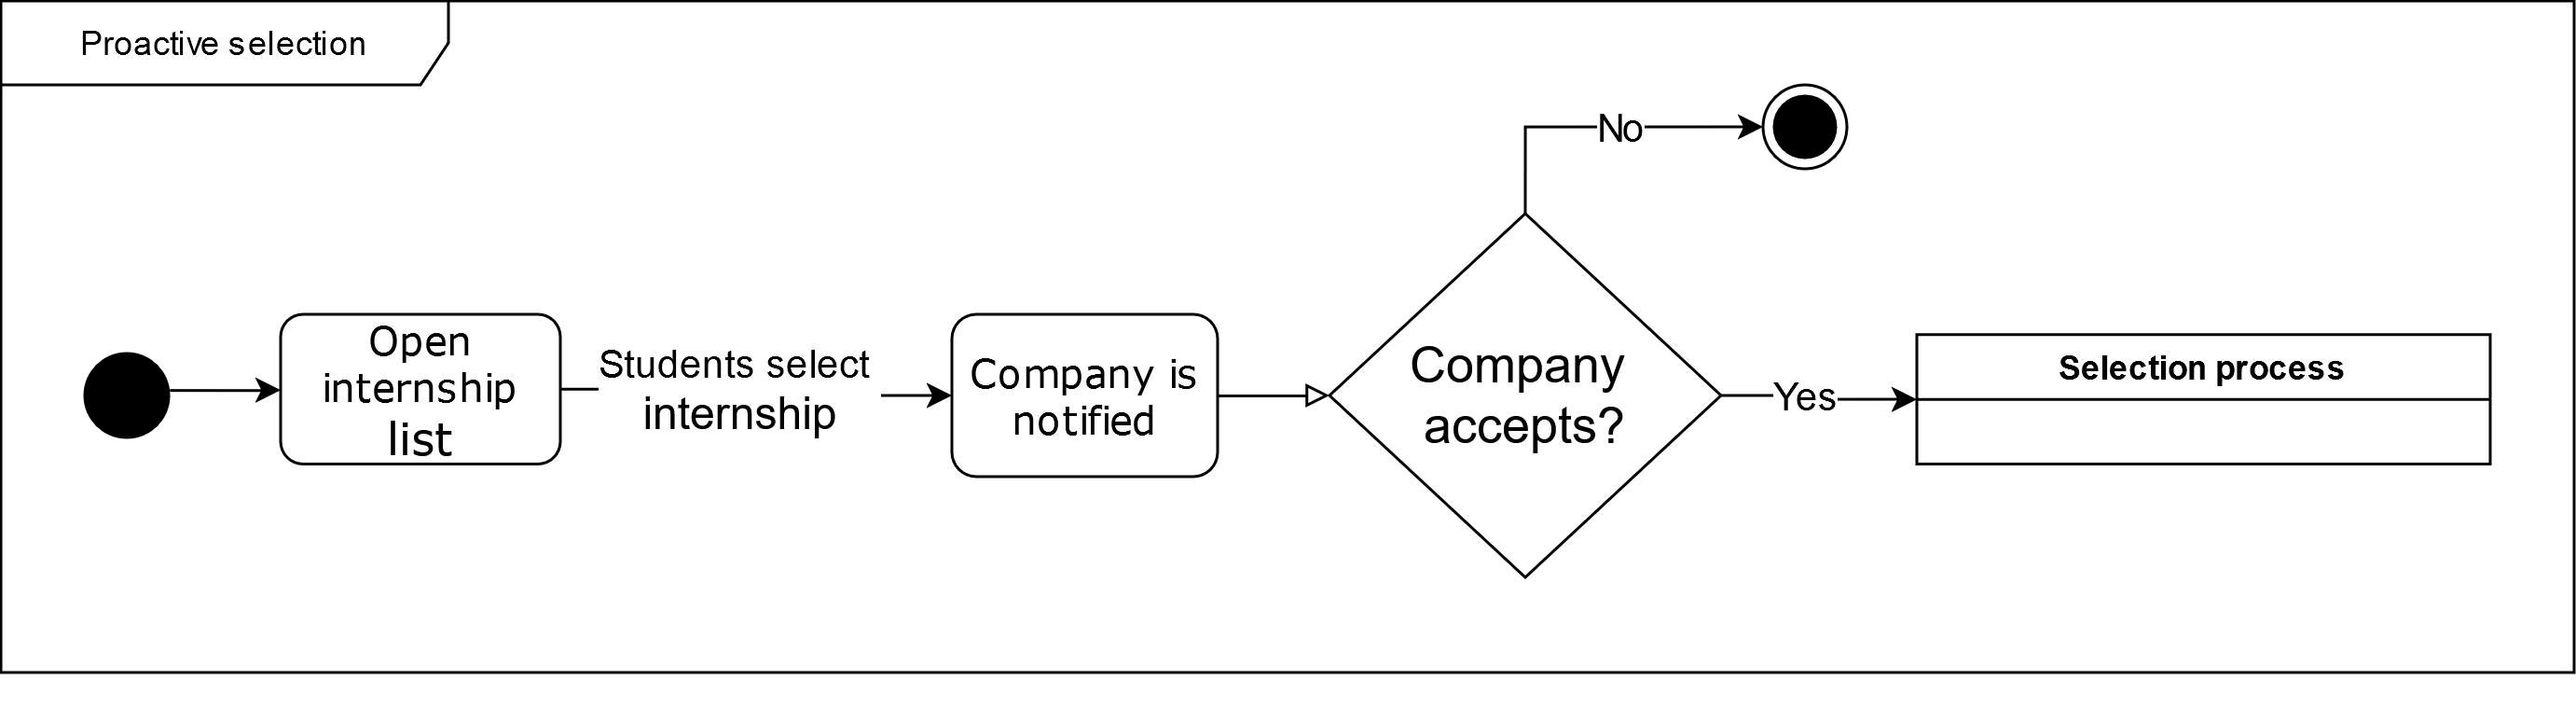
\includegraphics[width=\textwidth]{Images/Proactive selection.png}
    \caption{Proactive selection}
    \label{Proactive selection}
\end{figure}
This state diagram describes the process of manual selection of the internship by the student. In the initial state, the "Open internship list" the system is displaying some internship, and the student can select one of them, when is selected the system goes into the "Company is notified" state and notify the company interested, that can accept or not the request, in case of acceptance, the selection process start. 
\begin{figure}[H]
    \centering
    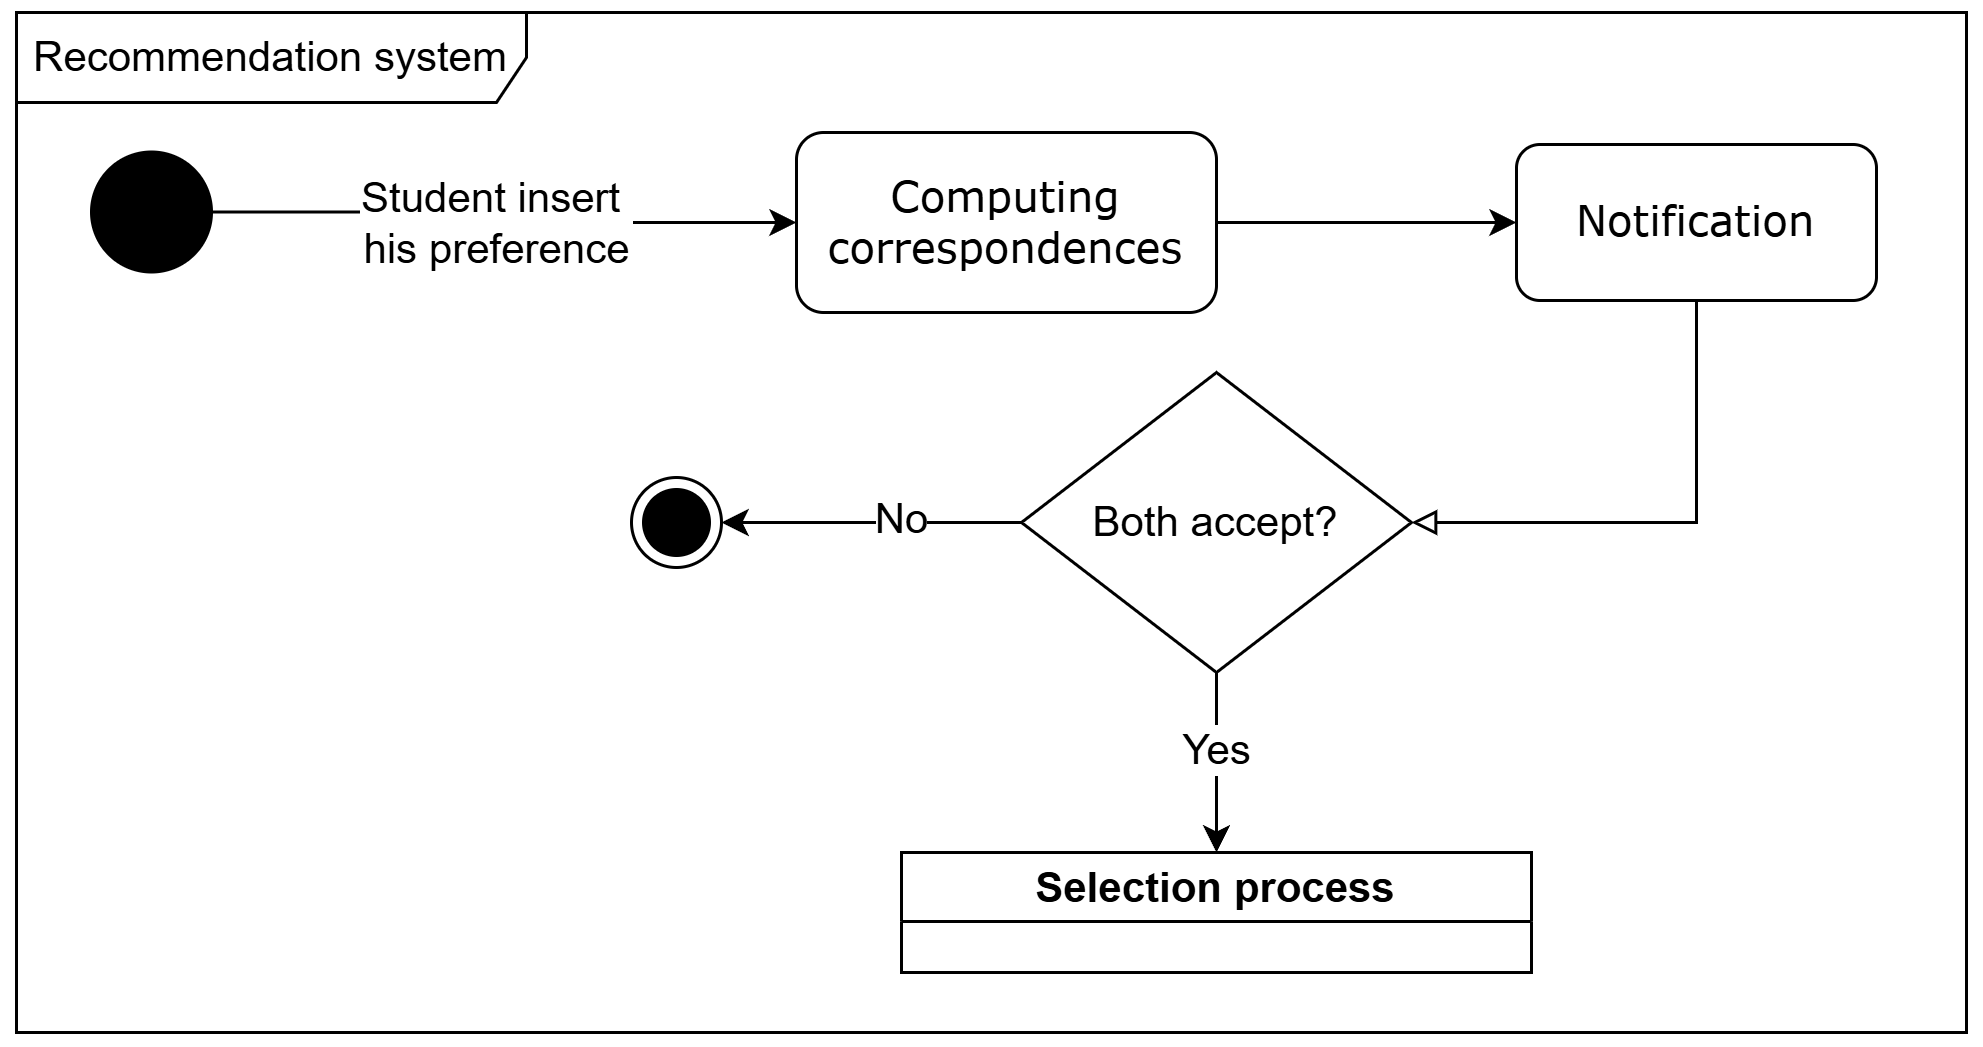
\includegraphics[width=\textwidth]{Images/Recommendation system.png}
    \caption{Recommendation process}
    \label{Recommendetion system}
\end{figure}
After the insertion of the preferences by the student, the system goes to the state of "computing correspondences" where it actually search for an internship that can match with the preferences of a company, through a keyword search of the preferences through the CVs' content or a statistical analysis of the internships. The system always found the best match, then proceed to the state of "notification" where it notify both the counterparts, if both of them accept, then the system proceed with the selection process, else the selection process never start.
\begin{figure}[H]
    \centering
    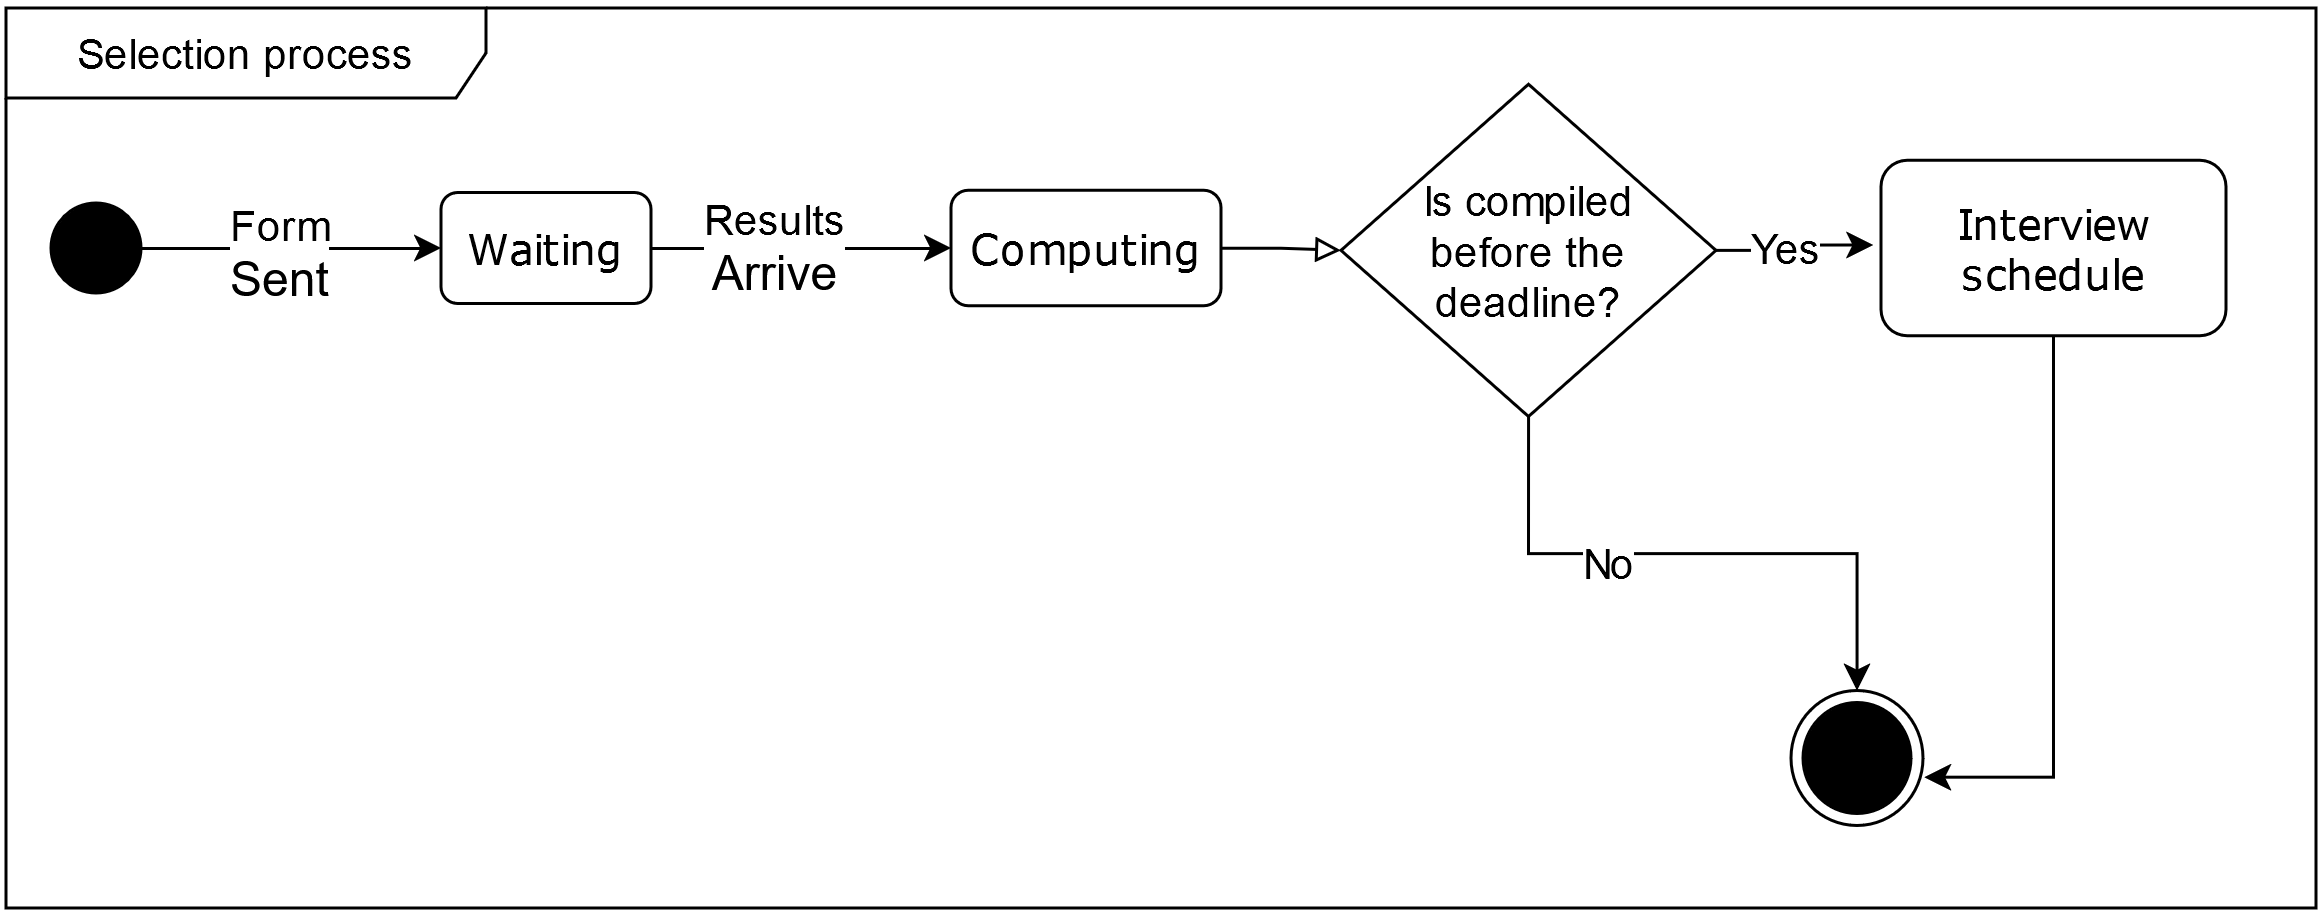
\includegraphics[width=\textwidth]{Images/Selection process.png}
    \caption{Selection process}
    \label{Selection process}
\end{figure}
This state diagram describe the selection process, once it starts, the system sent a form and goes to the "Waiting" state, where it waits until the student compile the form and send back the results, Then when they arrive, it goes to the "Computing" state and elaborate the form result and if the date of compiling is before the deadline, the system proceeds with the scheduling of the interview in the "Interview schedule" state, where it also produce the link for the video interview. 

\subsection{Product functions}
The following sections contains the main product function of S\&C.
\begin{itemize}
    \item \textbf{Sign and Login}\\
    These functions will be available to all the users. The sign-up functionality allows users to create an account to register themselves to the platform. Each user will be asked to select if he/she is a student or a company and provide own data such as name, email and password; for the student will also be asked surname, his/her description and CV, for the company the VAT number and a description of itself. The login functionality allows users to access an existing account using the credentials (email and password) chosen at registration. 
    \item \textbf{Managing internships and data}\\
    This function allows companies to insert their offers into the platform, it requires a name, a start and an end date, if there is one, a salary, the qualification required and a description. Also a company can modify the existent one and its data.
    \item \textbf{Managing student data}\\
    This function allows a student to insert his/her updated data.
    \item \textbf{Autonomous research}\\
    This function allows a student to search throughout all the internships available and find what suits him better and he/she ask the company to start the selection process. He/She can search through the list with a keyword or through the application of some filter. 
    \item \textbf{Recommendation system}\\
    This function search for a correspondence between the student and the companies, taking in consideration the CV of the student, the preferences and the description of both. If this search fails, it takes in consideration a statistical analysis approach that produce the most suitable match from the list of internships.
    \item \textbf{Selection process}\\
    This function handle the selection process, once all the parts have accepted to collaborate, S\&C sends a form to the student, and when the student send it back, it check if it has done in time, if yes, schedules an interview for the first spot available for both the student and the company, else it ends the process. The function will end after the acceptance or not by the company of the student after the interview. 
\end{itemize}

\subsection{User characteristics}
Here it is provided a more detailed characterization of the two different types of users of the platform, also specifying the roles they can assume in different contexts. 
\begin{itemize}
    \item \textbf{Student}\\
    A student can be whoever wants to search for an internship and his/her is a real university student. After his/her registration, he/she gets the functionalities which are reserved for student such as managing data and autonomously searching for an internship.
    \item \textbf{Company}\\
    A company can be whoever wants to offer an internship. After its registration, it gets the functionalities which are reserved for companies such as managing data and offers for an internship.
\end{itemize}

\subsection{Assumptions, dependencies, and constraints}
\textbf{[A1]:} The user always selects the correct option about his/her/its position (student/company)\\
\textbf{[A2]:} All users have an active email address.\\ 
\textbf{[A3]:} All users have access to an internet connection\\
\textbf{[A4]:} A student is a real student, subscribed to a University.\\
\textbf{[A5]:} All users have a Zoom account.\\
\textbf{[A6]:} All Companies are real companies, and the inserted VAT number can be verified.\\
\textbf{[A7]:} The internship should start from a valid date, which is later from the interview date




Here is the command to refer to another element (section, figure, table, ...) in the document: \emph{As discussed in Section~\ref{sect:overview} and as shown in Figure~\ref{fig:metamodel}, ...}. Here is how to introduce a bibliographic citation~\cite{DAM}. Bibliographic references should be included in a \texttt{.bib} file.

\clearpage
{\color{Black}{\section{Specific Requirements}}}
\label{sect:Requirements}
\subsection{External Interface Requirements}
\subsubsection{User Interfaces}

The platform is featured with several Graphic User Interfaces such to allow all the different kinds of users to interact with all its functionalities. The most important ones are presented below: 
\begin{itemize}
    \item \textbf{Registration/Login Interface}\\
    This interface provides for two different forms to fill in personal data, either to register to the platform or to access the personalized Home Page. 
    \item \textbf{Home Page}\\
    In this page the student visualizes key information about the upcoming internship, and also inserts a keyword to search on them. If it is a company, it has the possibility to see its internship and notifications.
    \item \textbf{Profile page}\\
    With this interface, the user can review his/her personal data set during registration. 
    \item \textbf{Internships management}\\
    With this interface, a company can manage his own published internships and add new ones.
    \item \textbf{Internships feedback}\\
    With this interface, users can give feedback after completion of an internship and visualize all the given ones.
\end{itemize}
\subsubsection{Hardware Interfaces}
The platform does not provide any hardware interface since it is primarily a platform to find a internship: it does not require any external component or device other than the one it runs
on. 
\subsubsection{Software Interfaces}
The software, through an appropriate API, communicates with Zoom to manage the interview call. 
\subsubsection{Communication Interfaces}
The platform exploits the internet connection for communication to the main server, 
whose role is to manage all back-end functions such as storing data, responding to deadlines, and so on. 


\subsection{Functional Requirements}
\subsubsection{Use case diagrams}
In this section, some of the most significant Use Cases for S\&C platform have been represented, dividing them into two groups, one for each category of user.
\begin{figure}[H]
    \centering
    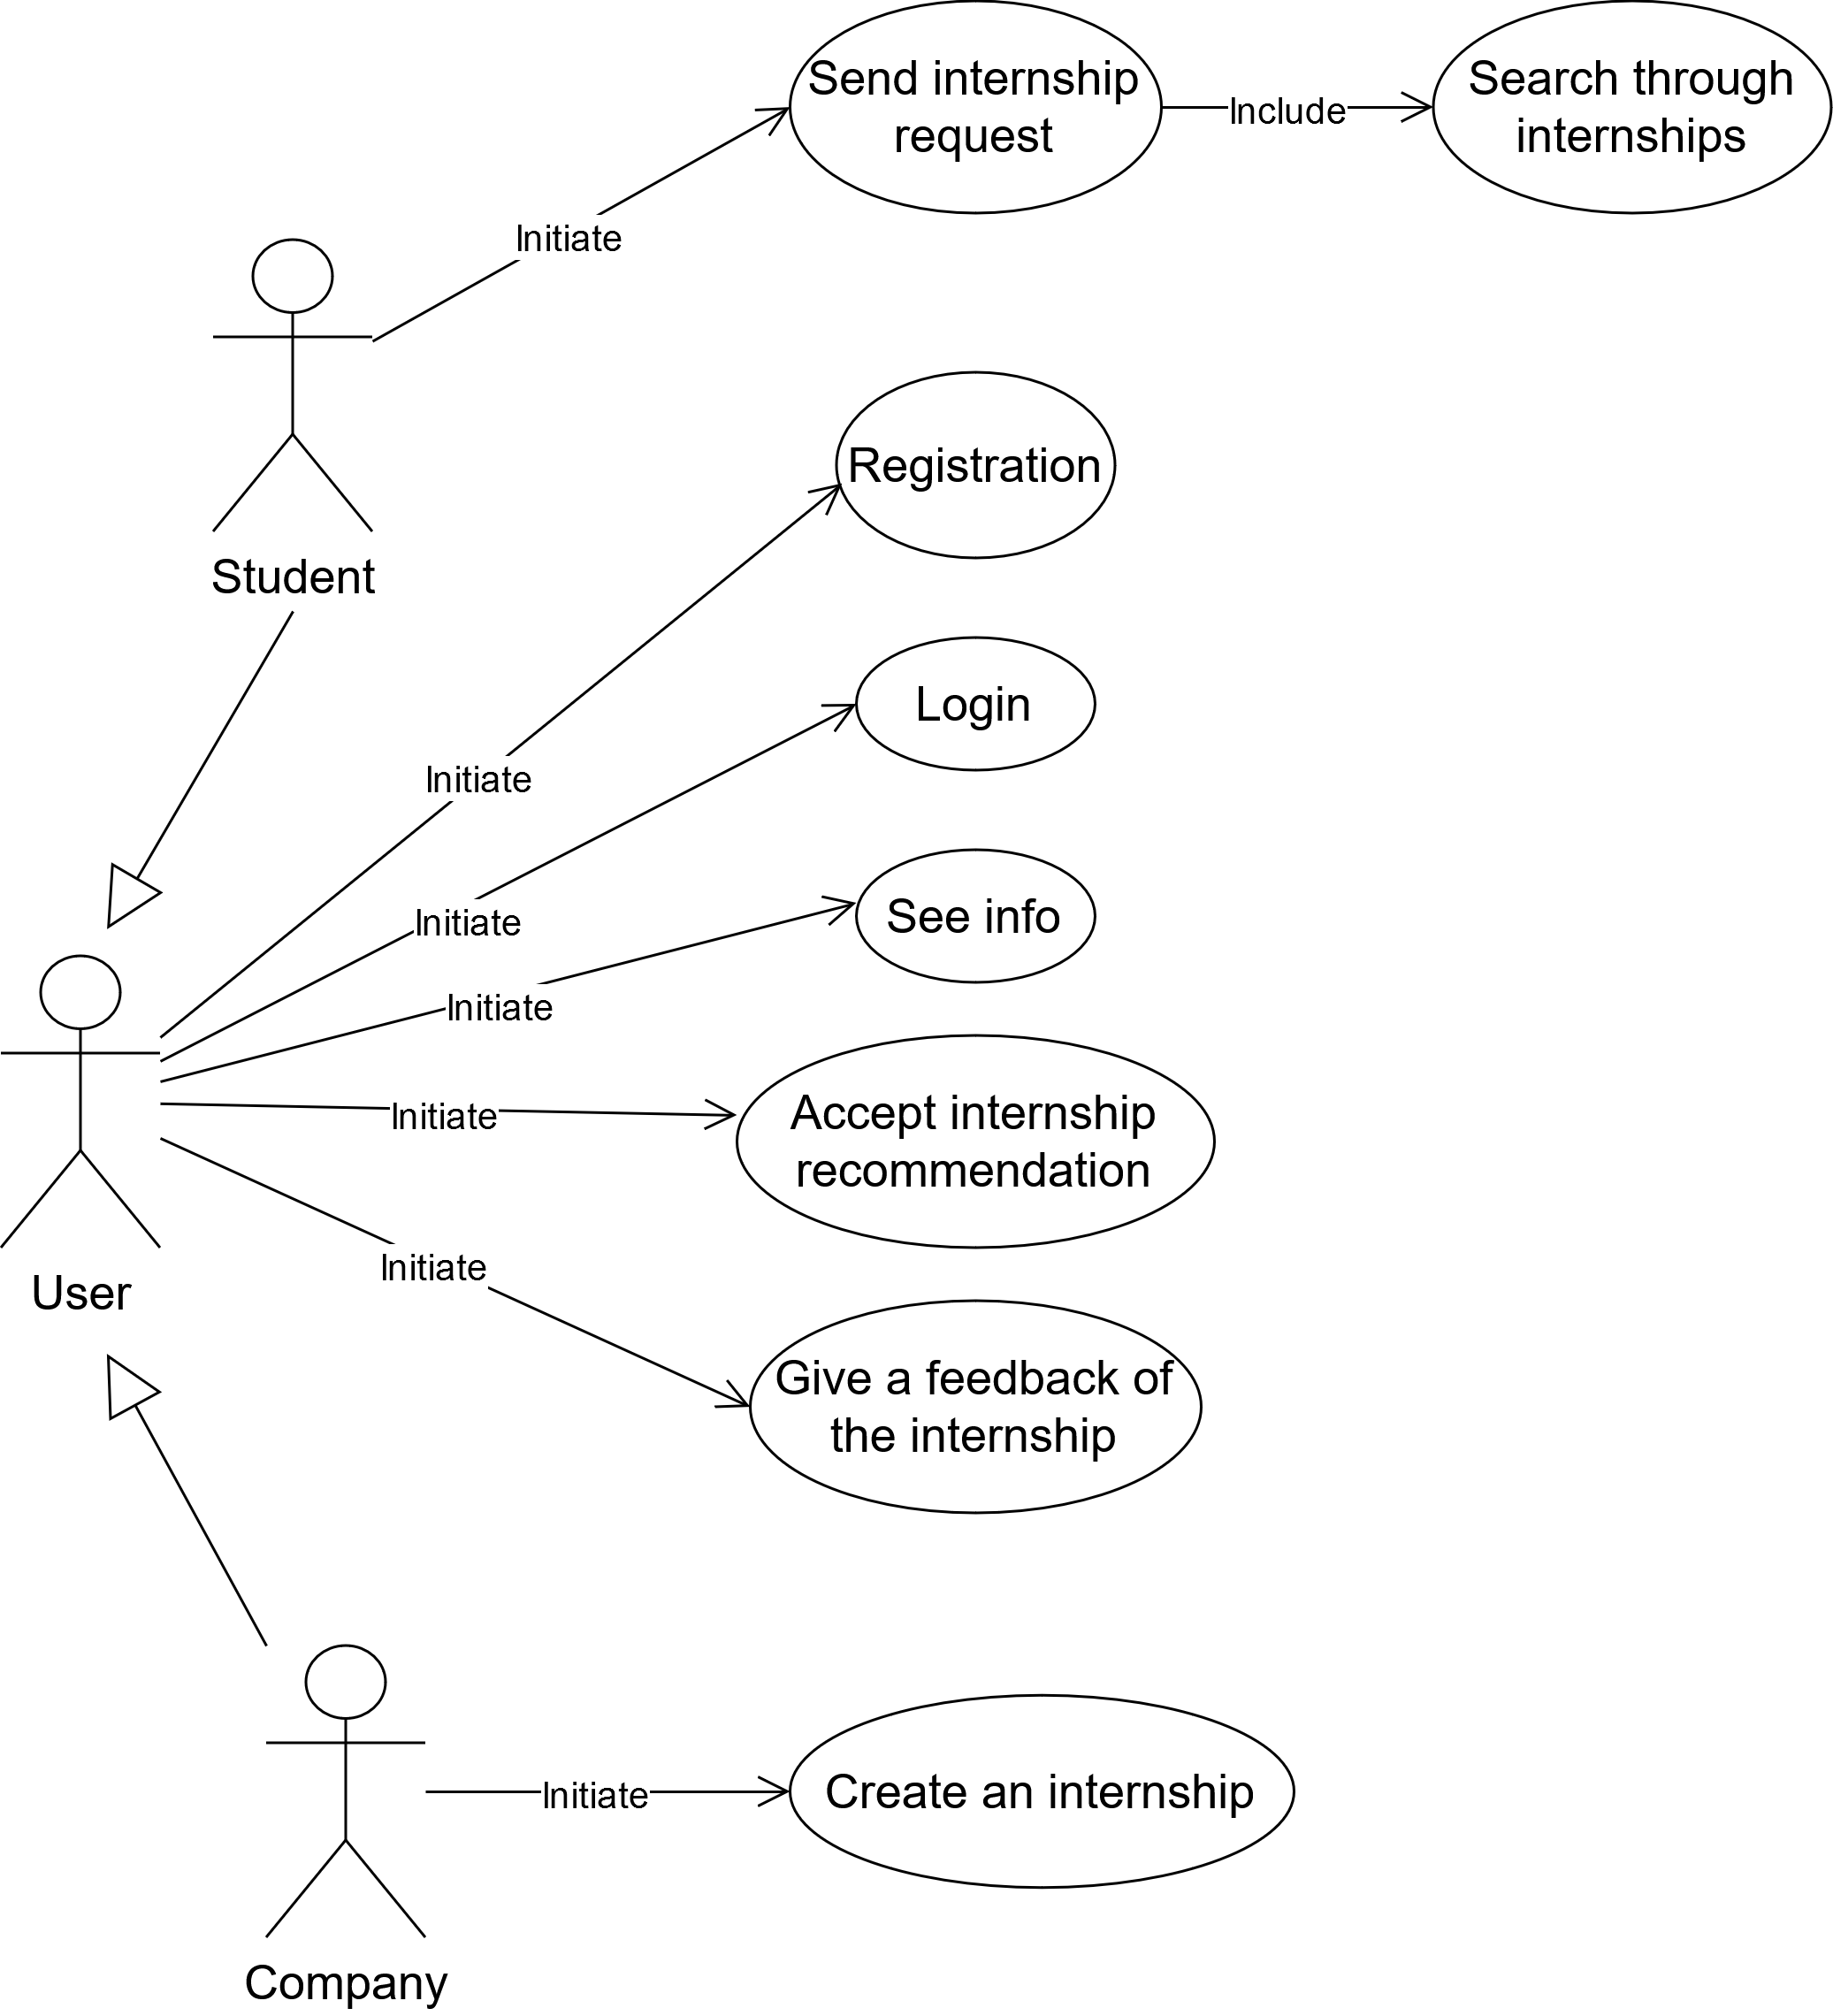
\includegraphics[width=0.75\linewidth]{Images/UseCasesDiagrams.png}
    \caption{Use Cases Diagram}
    \label{Use Cases Diagram}
\end{figure}\subsubsection{Use cases and related diagrams}

%uc1
\begin{table}[H]
\renewcommand\arraystretch{1.25}
    \centering
    \begin{tabular}{|l|p{12cm}|}
        \hline
        \textbf{Name} & Register user\\
        \hline
        \textbf{Actors} & User\\
        \hline
        \textbf{Entry conditions} & User has opened the platform\\
        \hline
        \textbf{Event flow} & 
        \begin{enumerate}
            \item The User requests to register.
            \item The system asks the user to choose if it is a Student or a Company and to provide relative data.
            \item User submits all necessary information.
            \item The system checks if email has been already used by another user to register.
            \item System updates the database with the User’s information and displays a message of confirmed registration. 
        \end{enumerate}\\
        \hline
        \textbf{Exit conditions} & User has successfully registered \\
        \hline
        \textbf{Exception} & User provides an email already registered in the database. The system displays an error.\\
        \hline
    \end{tabular}
    \caption{UC1}
    \label{UC1}
\end{table}

\begin{figure}[H]
    \centering
    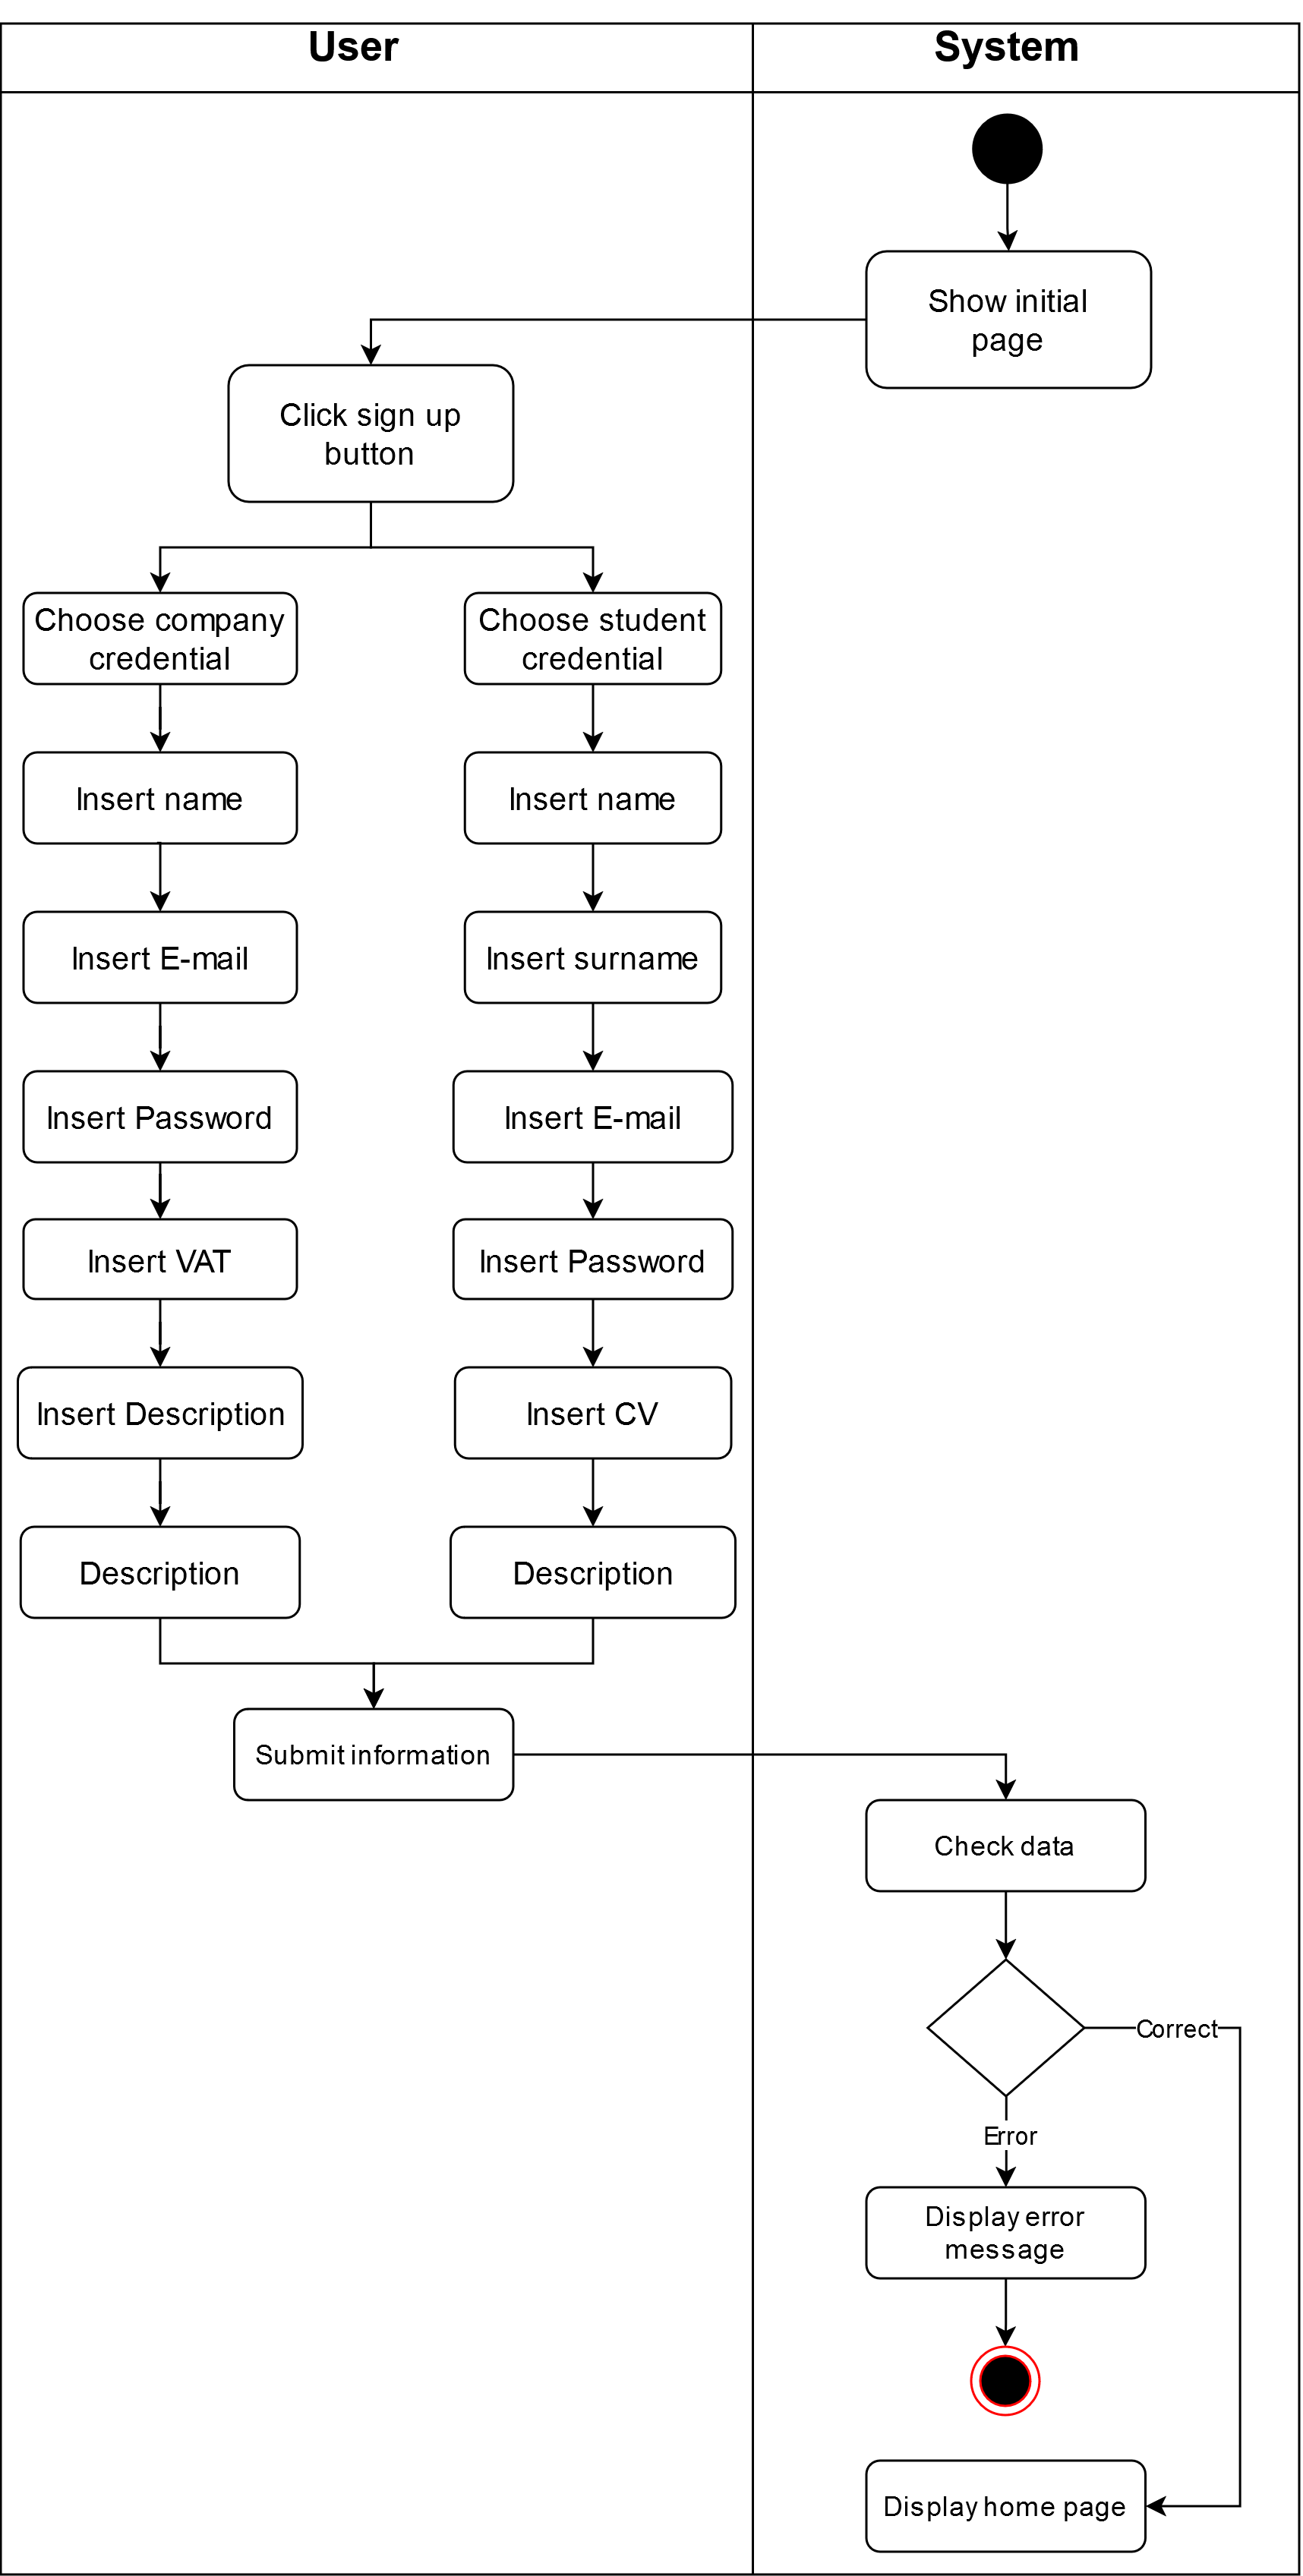
\includegraphics[width=0.75\linewidth]{Images/UseCasesDiagrams-Register.png}
    \caption{AD1}
    \label{AD1}
\end{figure}

%uc2
\begin{table}[H]
\renewcommand\arraystretch{1.25}
    \centering
    \begin{tabular}{|l|l|}
    \hline
    \textbf{Name} & Login user\\
    \hline
    \textbf{Actors} & User\\
    \hline
    \textbf{Entry conditions} & User has registered to the platform \\
    \hline
    \textbf{Events flow} &
    \begin{tabular}[c]{@{}l@{}}
    1. User inserts in apposite fields the credentials for logging in \\(username and password) and presses the “Login” button\\
    2. The system checks the correctness of the credentials inserted\\
    3. The system displays the home page\\
    \end{tabular}\\
    \hline
    \textbf{Exit conditions} & User is logged in \\
    \hline
    \textbf{Exception} & \begin{tabular}[c]{@{}l@{}}
    User inserts wrong combina
    tion of credentials and presses Login button.\\
    In this case, the application displays the Login page with an error\\
    \end{tabular}\\
    \hline
    \end{tabular}
    \caption{UC2}
    \label{UC2}
\end{table}

\begin{figure}[H]
    \centering
    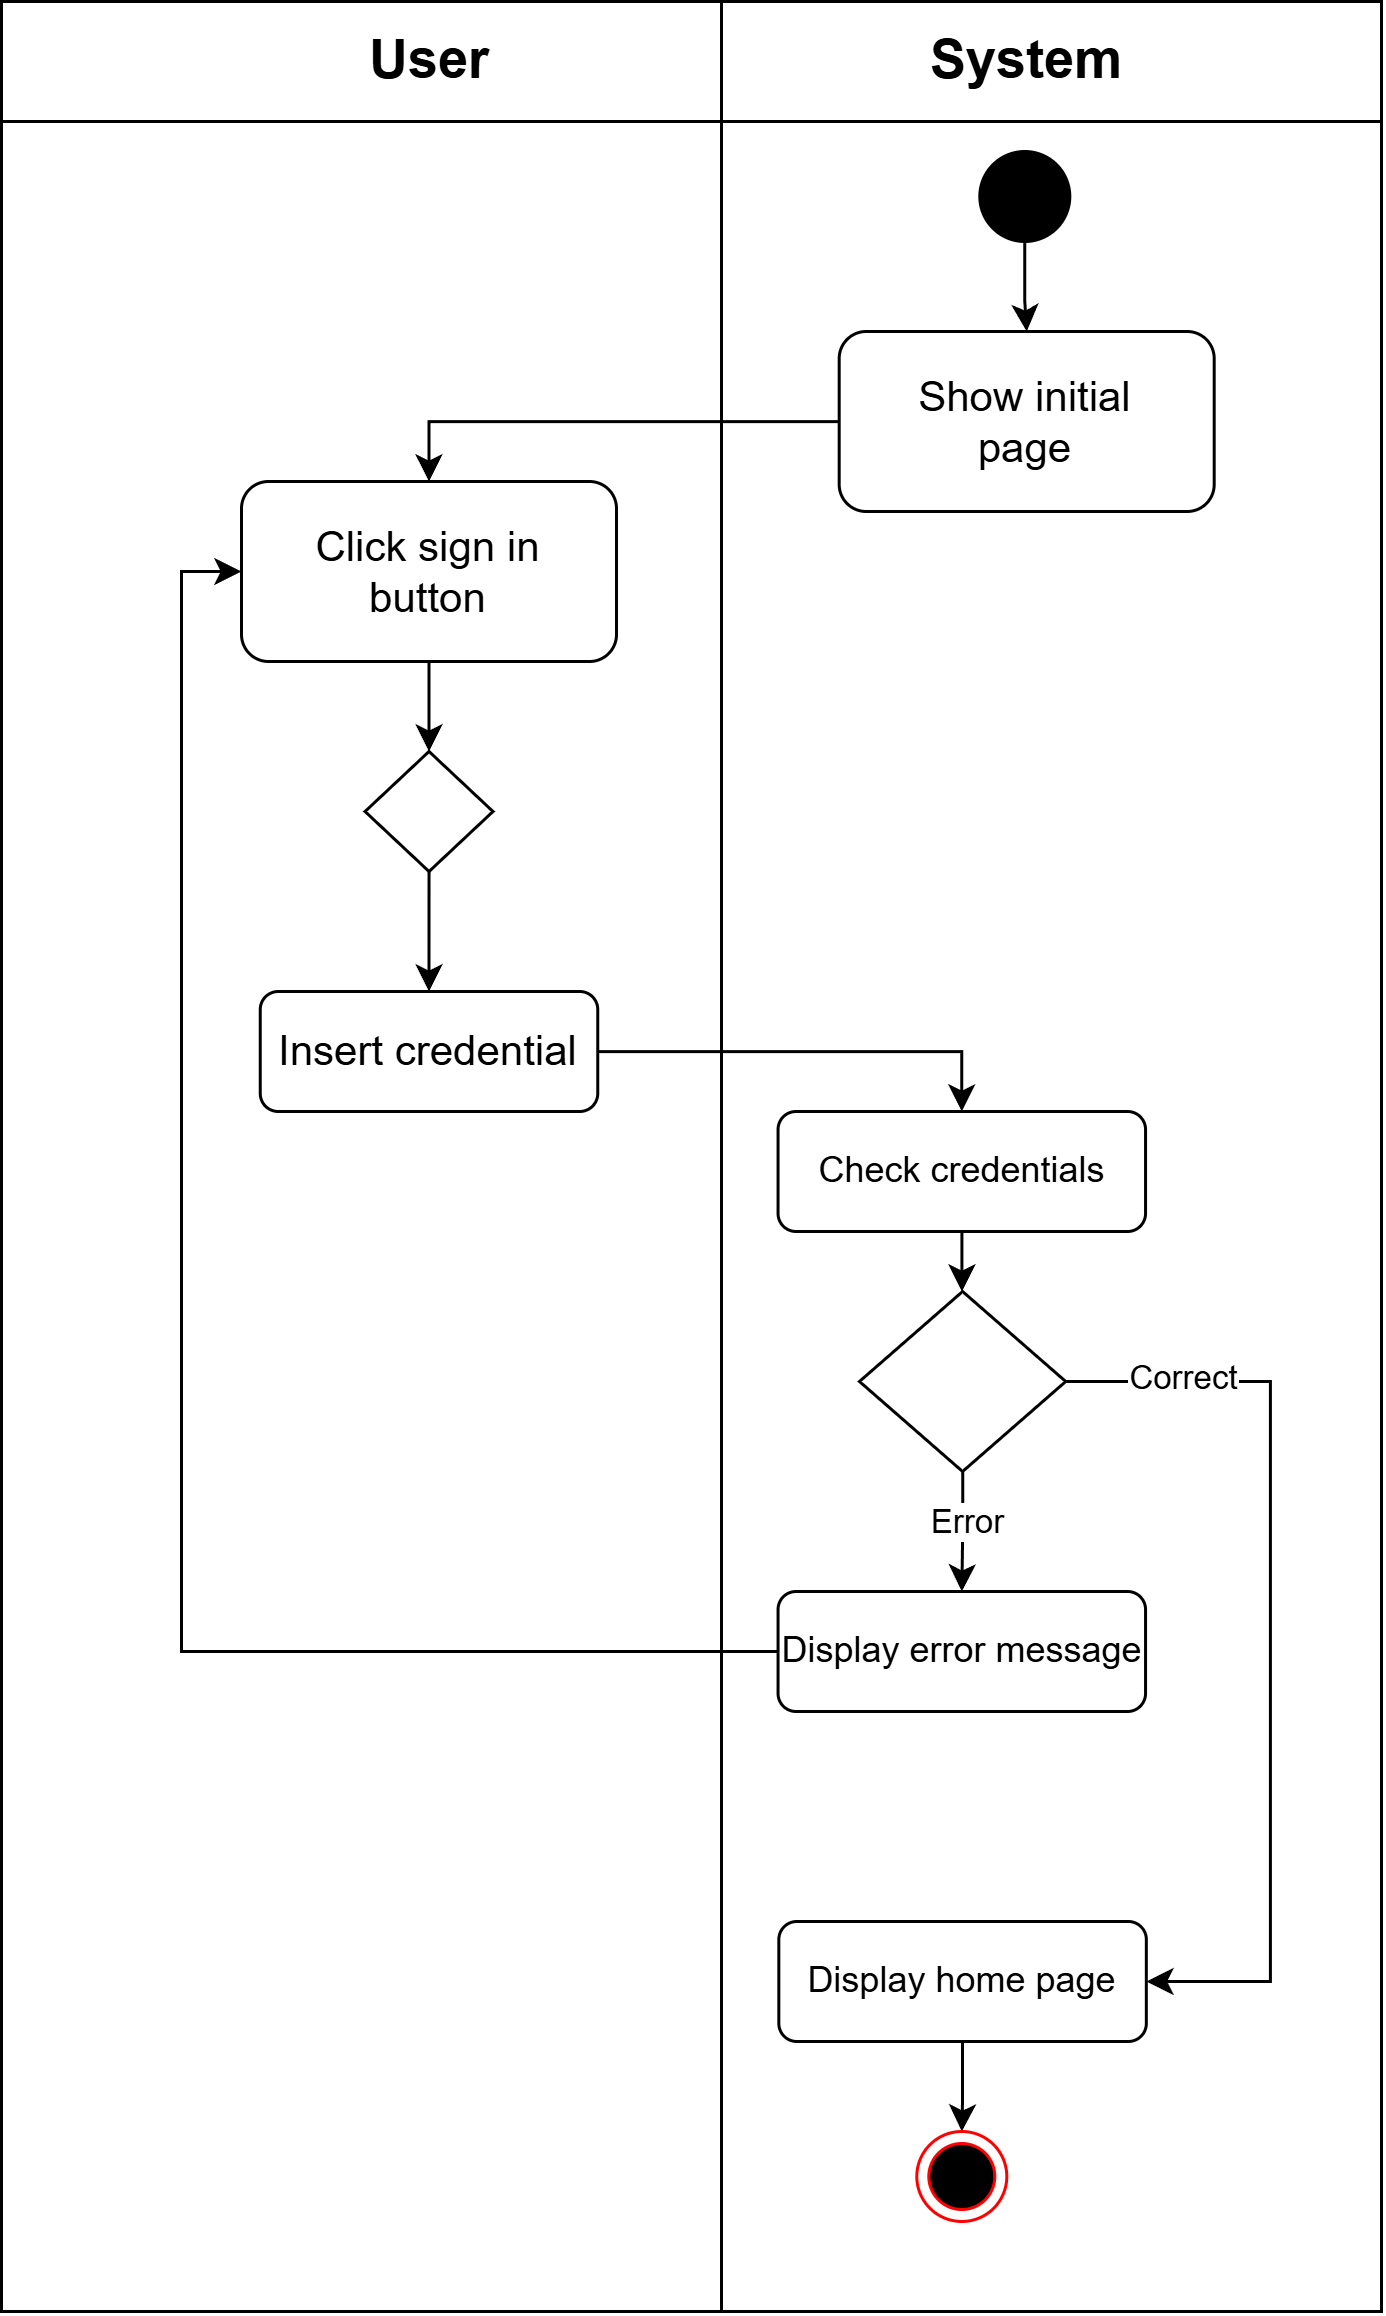
\includegraphics[width=0.75\linewidth]{Images/UseCasesDiagrams-Login.png}
    \caption{AD2}
    \label{AD2}
\end{figure}

%uc3
\begin{table}[H]
\renewcommand\arraystretch{1.25}
    \centering
    \begin{tabular}{|l|p{12 cm}|}
    \hline
    \textbf{Name} & User data management\\
    \hline
    \textbf{Actors} & User\\
    \hline
    \textbf{Entry conditions} & User has logged in to the platform \\
    \hline
    \textbf{Events flow} &
    \begin{enumerate}
        \item System show home page.
        \item User click on button "My data".
        \item System show user data.
        \item User click on button "Modify data".
        \item User can modify its information.
        \item User click on button "insert".
        \item System check validity.
        \item System shows the data updated.
    \end{enumerate}\\
    \hline
    \textbf{Exit conditions} & Company insert a valid internship \\
    \hline
    \textbf{Exception} & \begin{tabular}[c]{@{}l@{}}
    User change e-mail, inserts a not valid one and presses insert button.\\
    In this case, the application displays the Home page with an error\\
    \end{tabular}\\
    \hline
    \end{tabular}
    \caption{UC3}
    \label{UC3}
\end{table}

\begin{figure}[H]
    \centering
    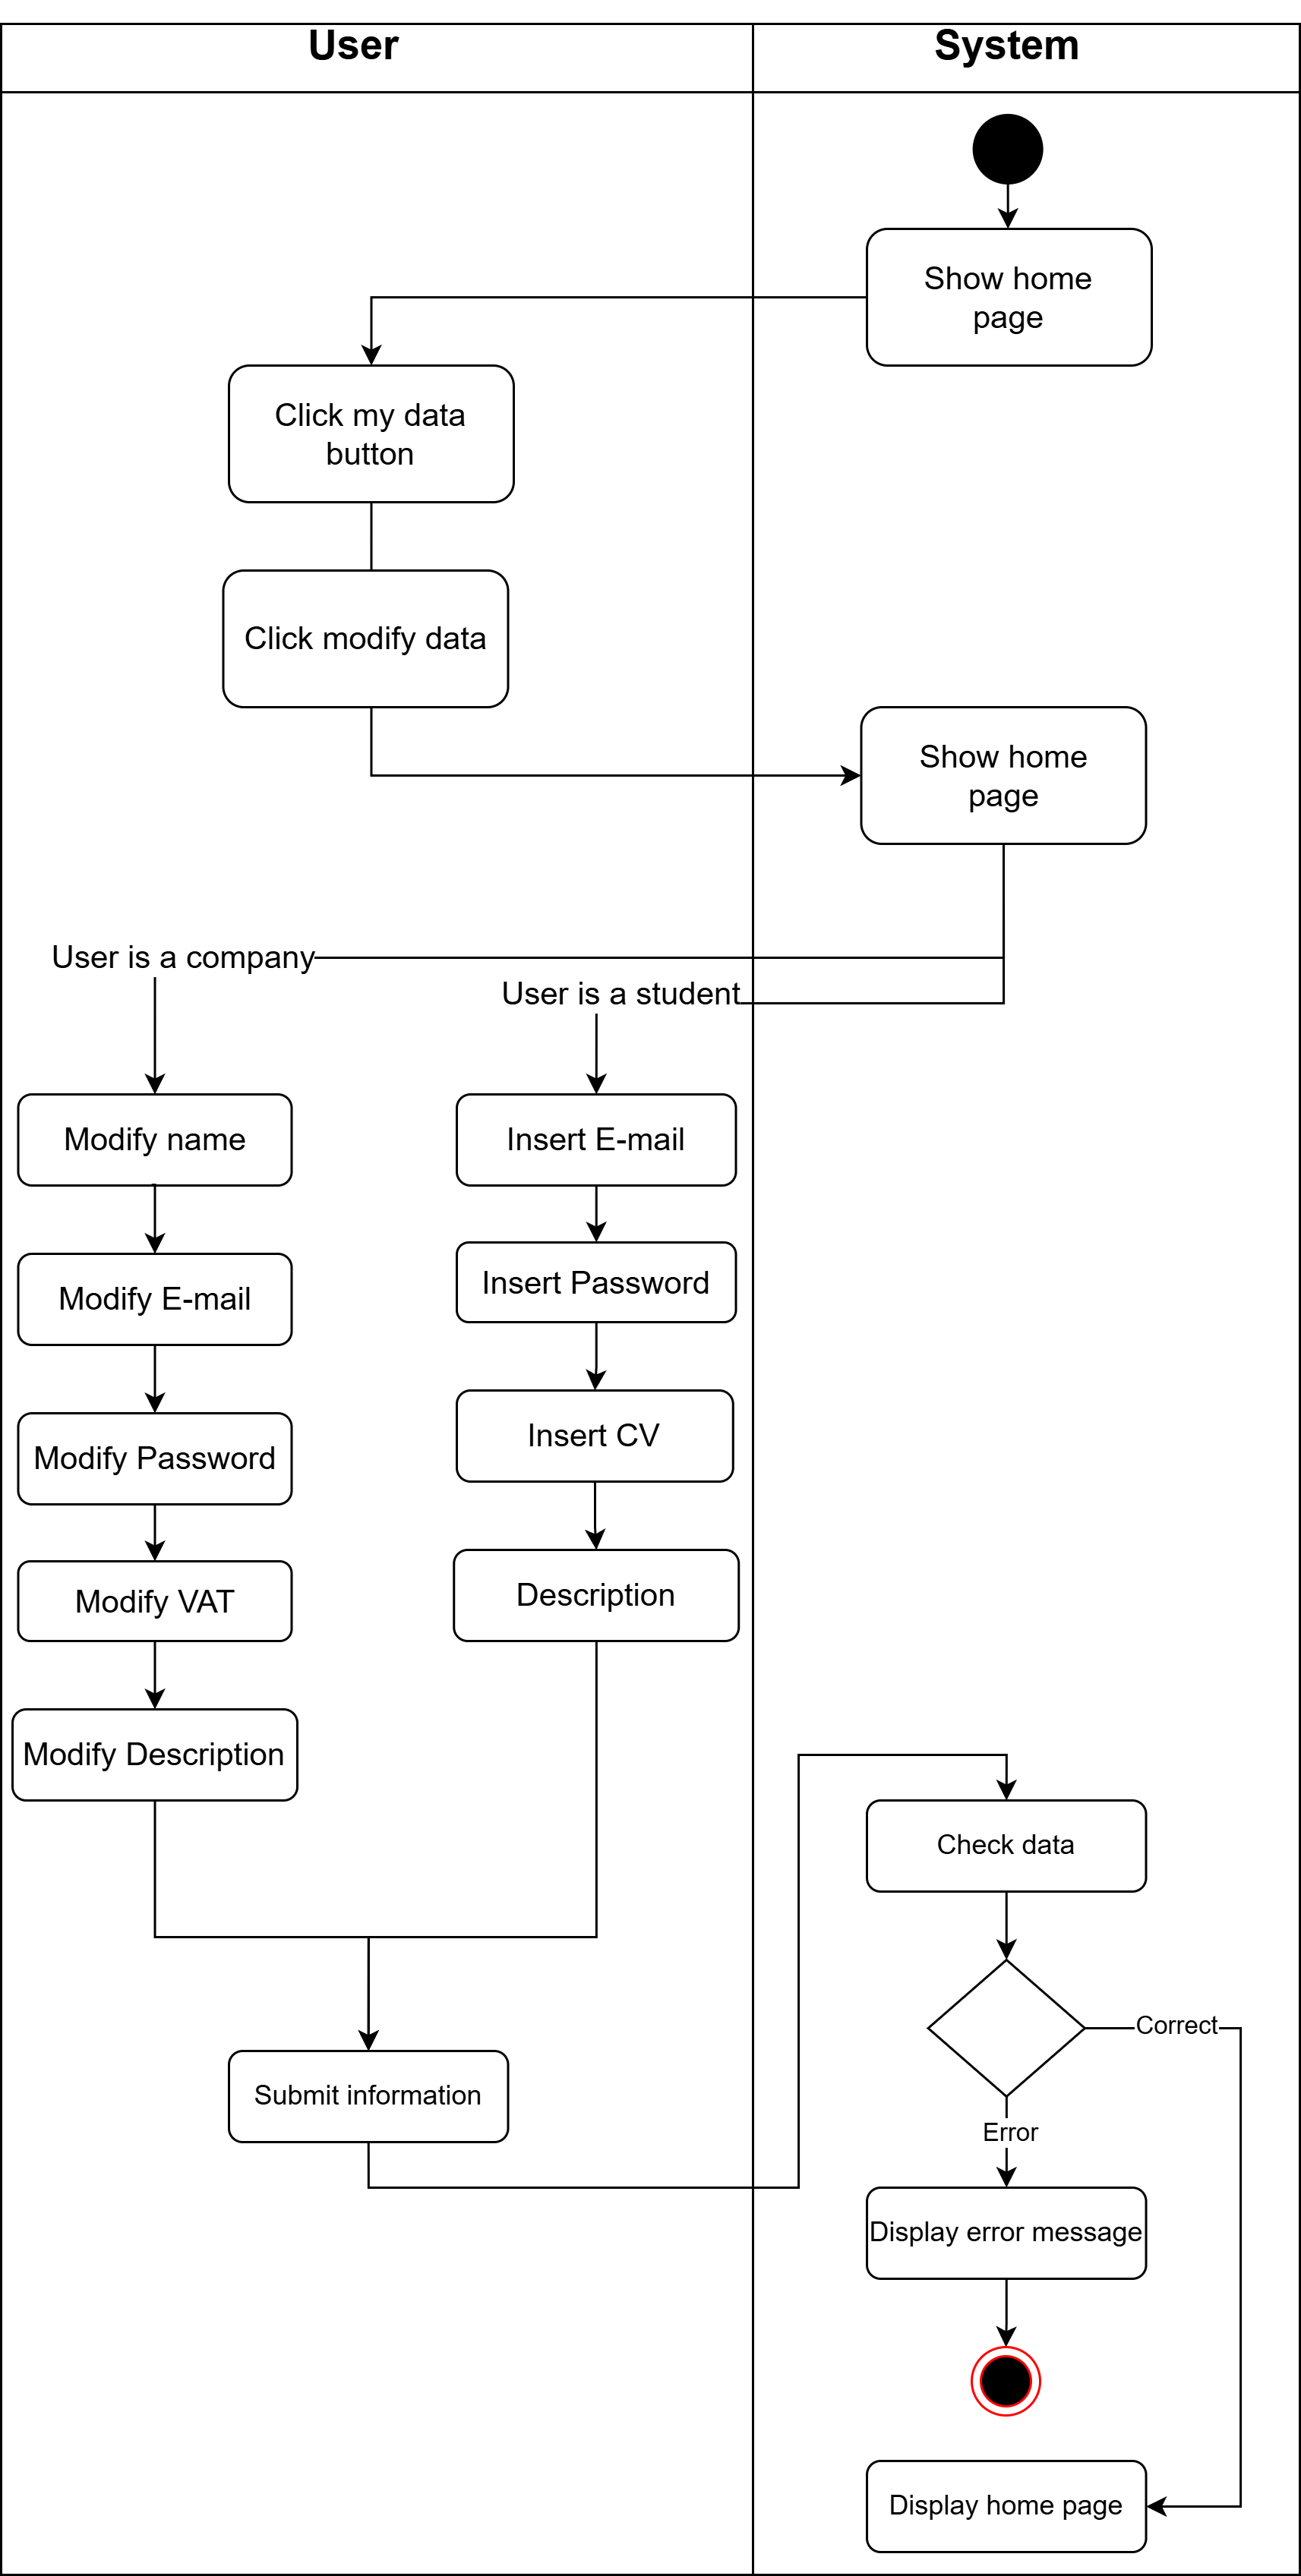
\includegraphics[width=0.7\linewidth]{Images/UseCasesDiagrams-manage-data.png}
    \caption{AD3}
    \label{AD3}
\end{figure}

%uc4
\begin{table}[H]
\renewcommand\arraystretch{1.25}
    \centering
    \begin{tabular}{|l|p{12 cm}|}
    \hline
    \textbf{Name} & Internship insertion\\
    \hline
    \textbf{Actors} & Company\\
    \hline
    \textbf{Entry conditions} & Company has registered/logged in to the platform \\
    \hline
    \textbf{Events flow} &
    \begin{enumerate}
        \item System show the home page.
        \item Company click on button insert "new internship".
        \item Company insert valid information of an "internship", such as name, start date, end date, salary, qualification required and a description.
        \item Company click on button "insert".
        \item System check validity.
        \item System shows the inserted internship list updated.
    \end{enumerate}\\
    \hline
    \textbf{Exit conditions} & Company insert a valid internship \\
    \hline
    \textbf{Exception} & \begin{tabular}[c]{@{}l@{}}
    Company inserts a not valid date and presses insert button.\\
    In this case, the application displays the Home page with an error\\
    \end{tabular}\\
    \hline
    \end{tabular}
    \caption{UC4}
    \label{UC4}
\end{table}

\begin{figure}[H]
    \centering
    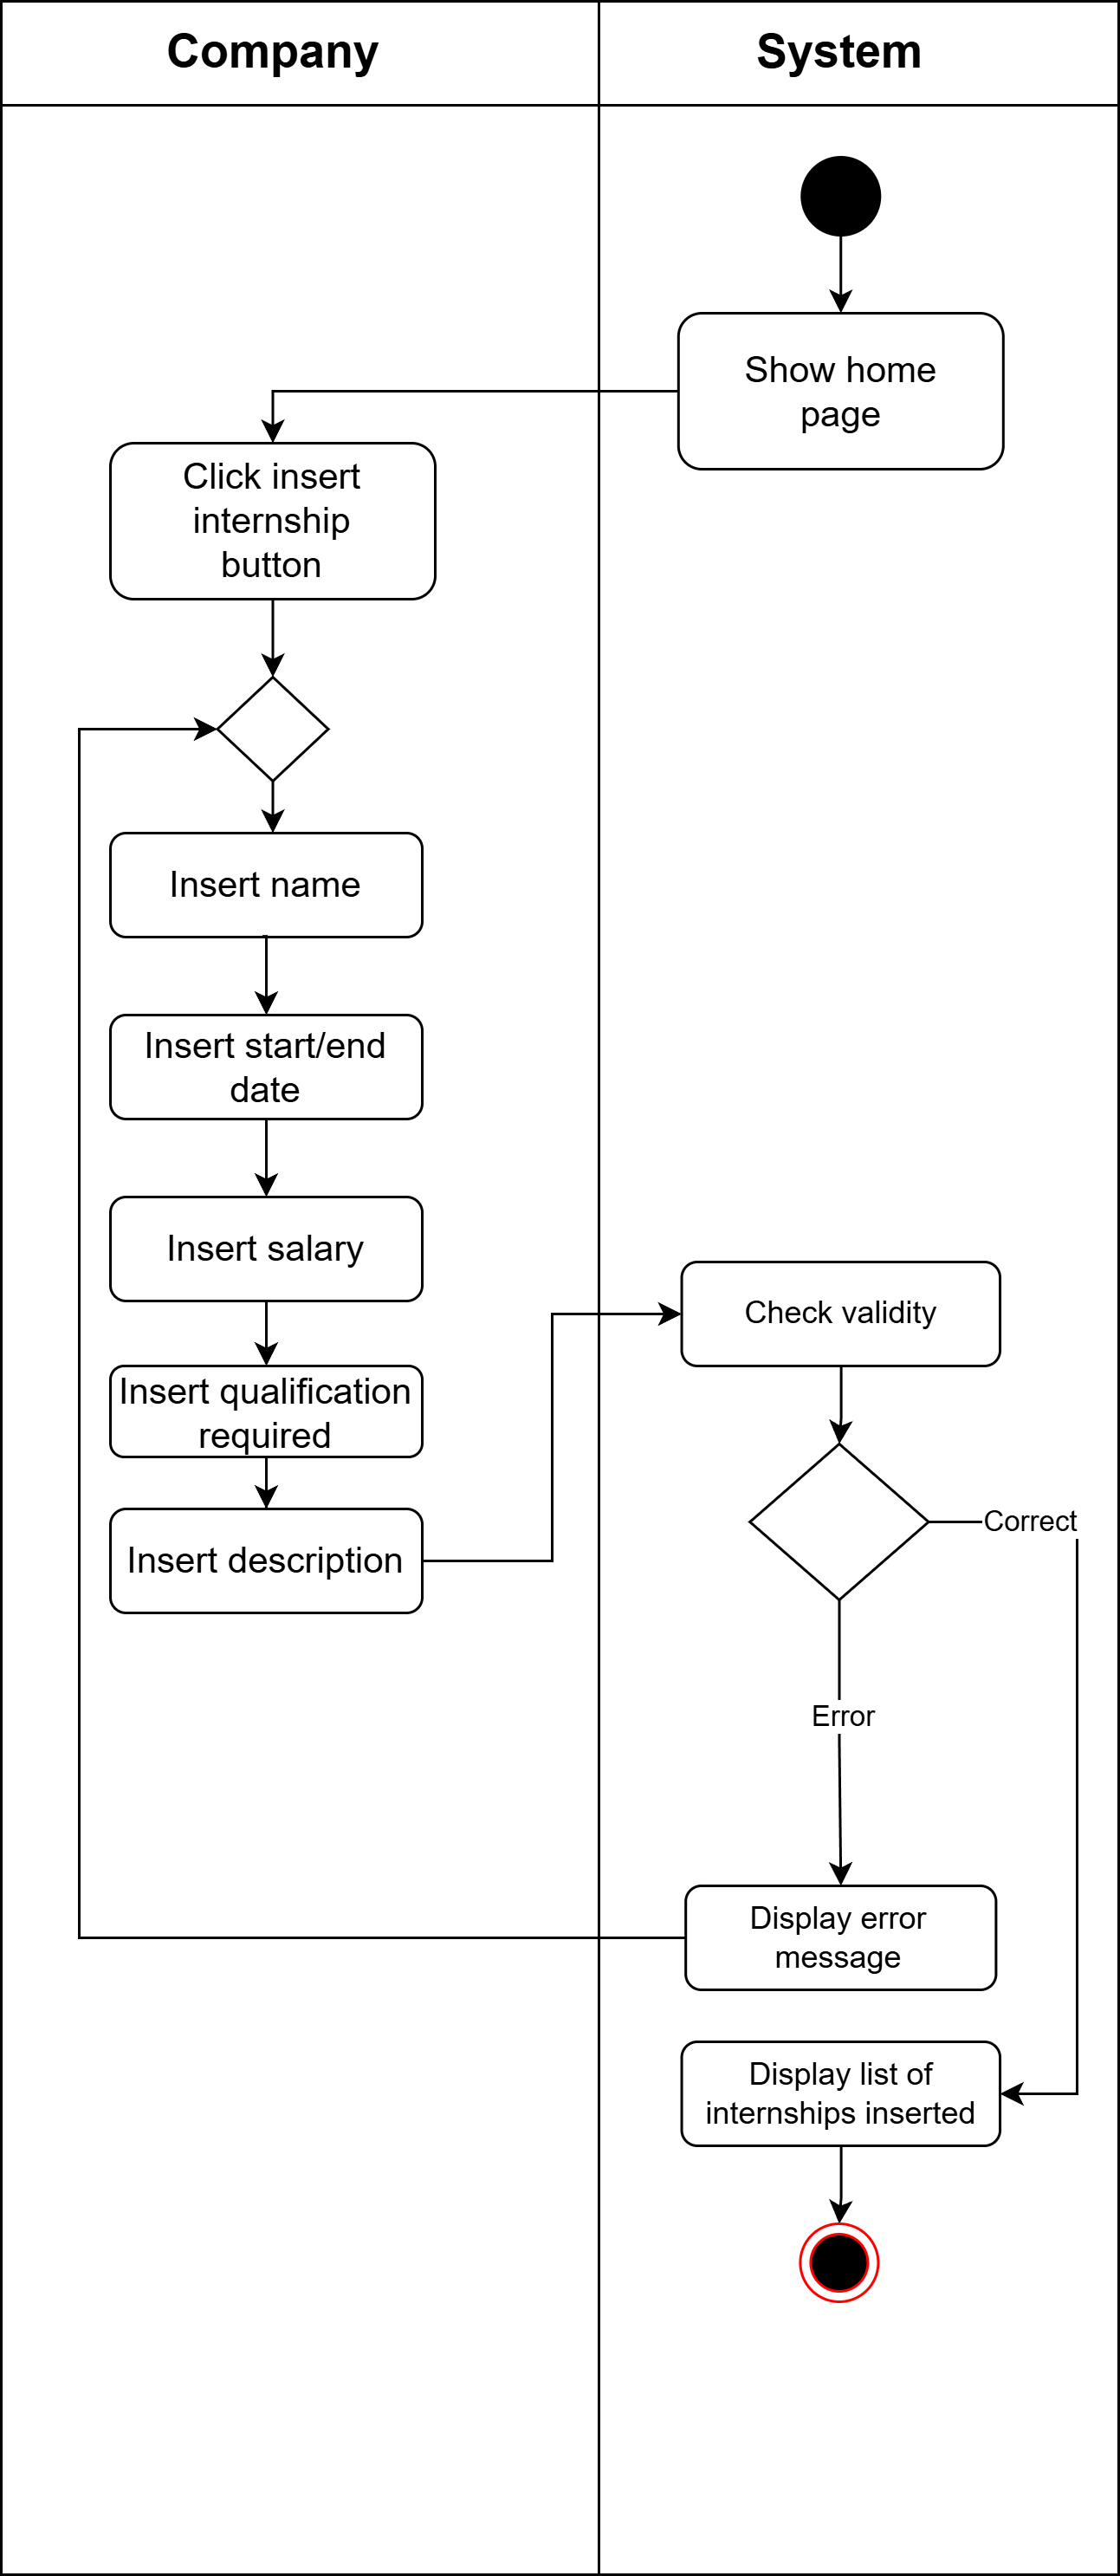
\includegraphics[width=0.65\linewidth]{Images/insert_internship.png}
    \caption{AD4}
    \label{AD4}
\end{figure}

%uc5
\begin{table}[H]
\renewcommand\arraystretch{1.25}
    \centering
    \begin{tabular}{|l|p{12 cm}|}
    \hline
    \textbf{Name} & Internship modification\\
    \hline
    \textbf{Actors} & Company\\
    \hline
    \textbf{Entry conditions} & Company has logged in to the platform \\
    \hline
    \textbf{Events flow} &
    \begin{enumerate}
        \item System shows home page.
        \item Company click on button "My internship".
        \item Company click on button "Modify internship".
        \item Company can modify information of an "internship", such as name, start date, end date, salary, qualification required and a description.
        \item Company click on button "insert".
        \item System check validity.
        \item System shows the inserted internship list updated.
    \end{enumerate}\\
    \hline
    \textbf{Exit conditions} & Company insert a valid internship \\
    \hline
    \textbf{Exception} & \begin{tabular}[c]{@{}l@{}}
    Company inserts a not valid date and presses insert button.\\
    In this case, the application displays the Home page with an error\\
    \end{tabular}\\
    \hline
    \end{tabular}
    \caption{UC5}
    \label{UC5}
\end{table}

\begin{figure}[H]
    \centering
    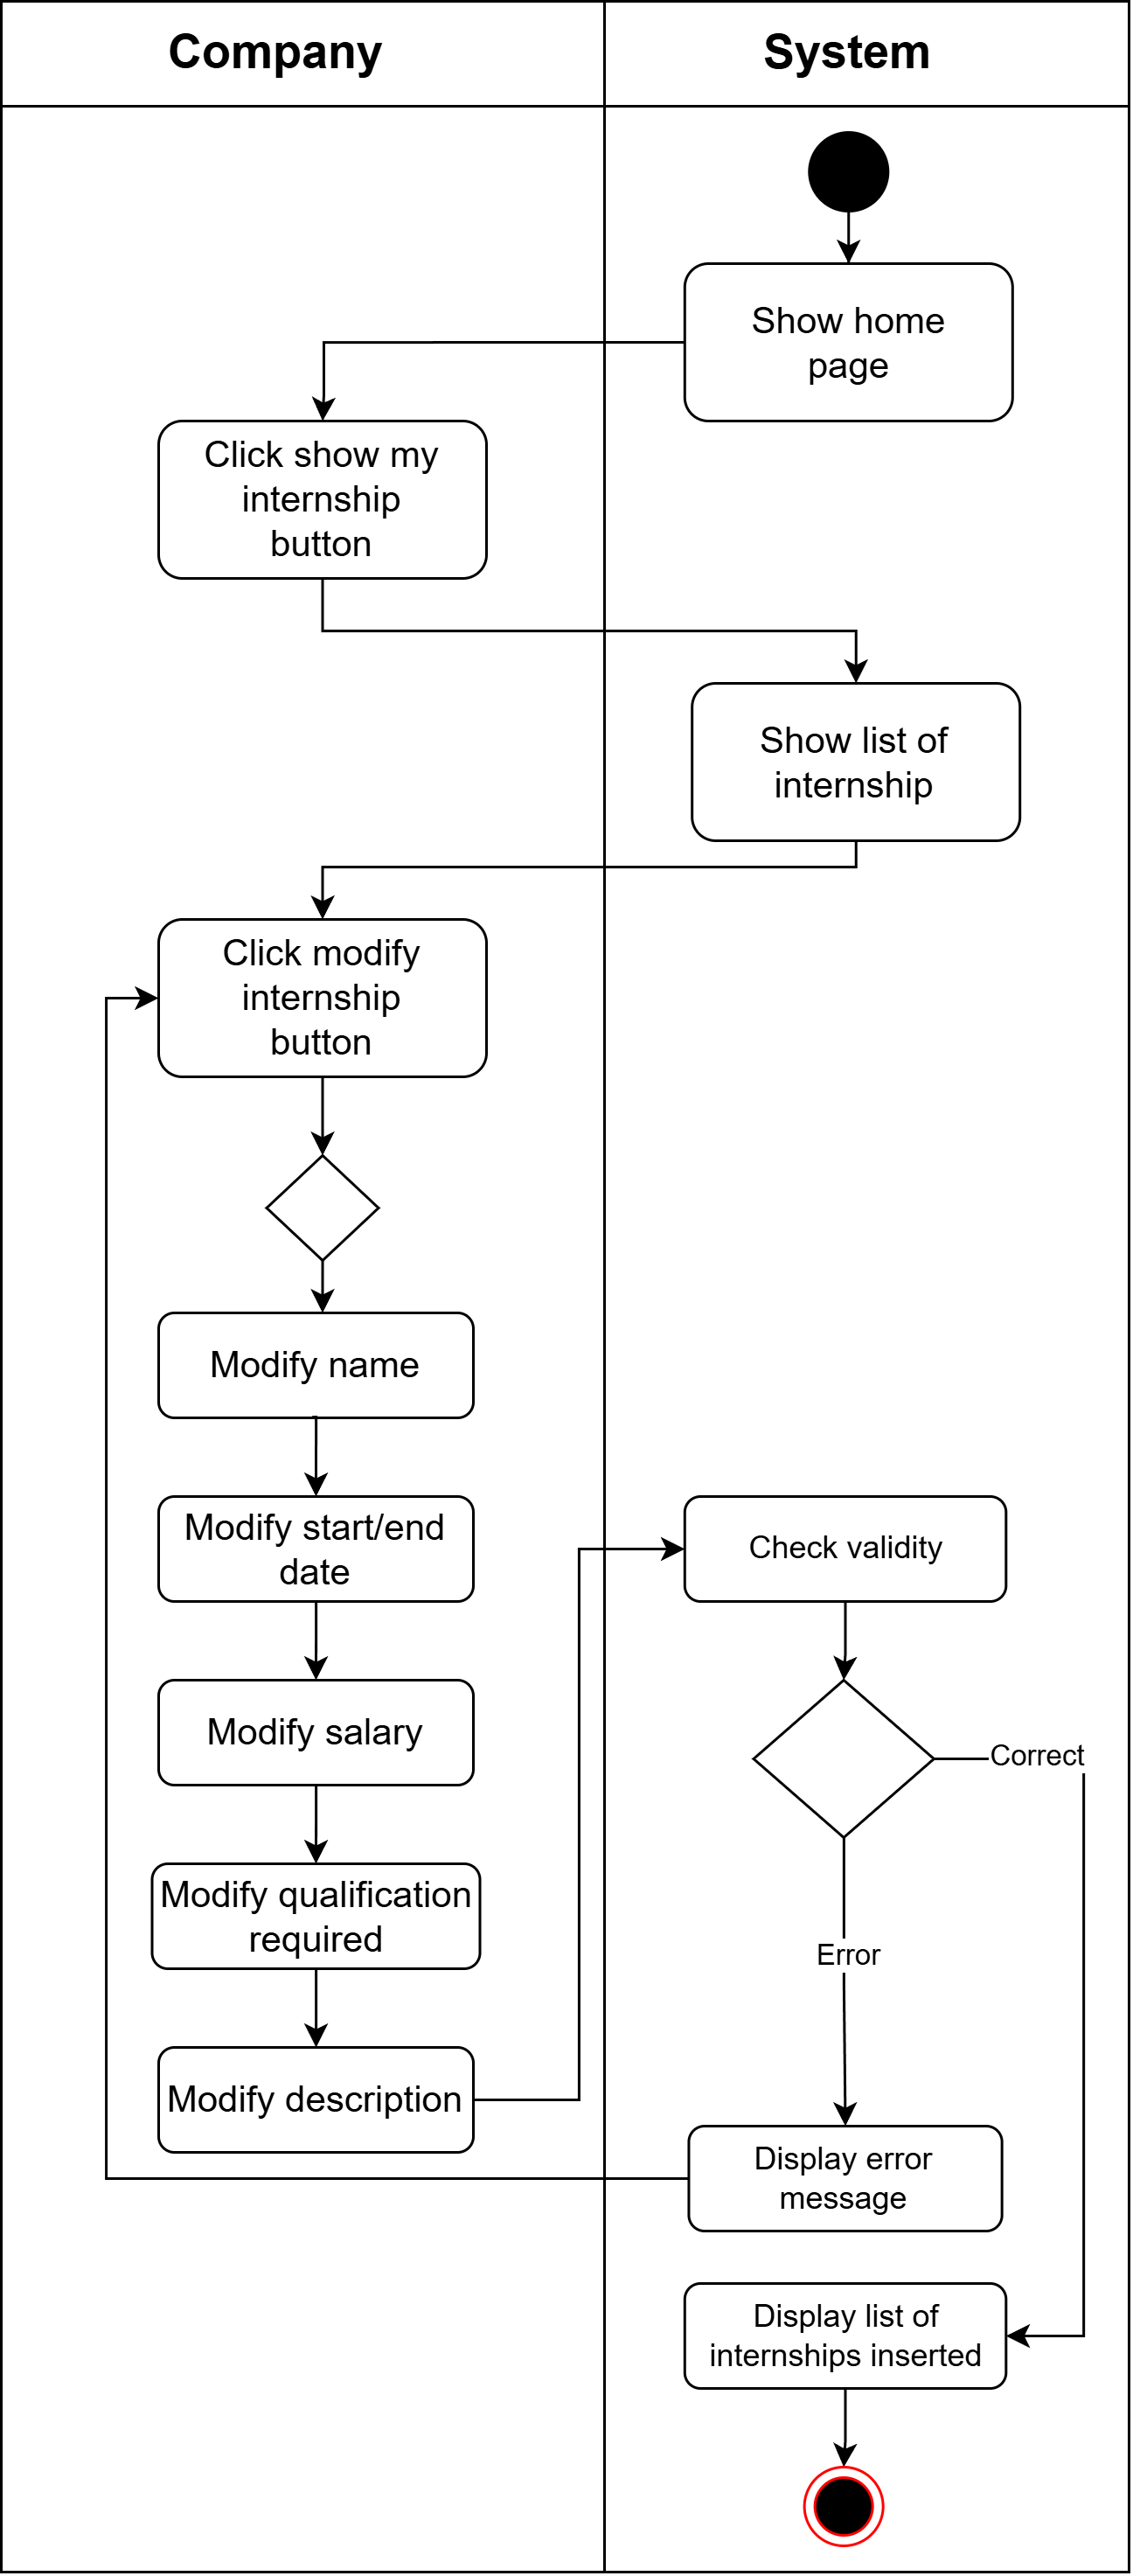
\includegraphics[width=0.6\linewidth]{Images/UseCasesDiagrams-UC modify-internship.png}
    \caption{AD5}
    \label{AD5}
\end{figure}

%uc6
\begin{table}[H]
\renewcommand\arraystretch{1.25}
    \centering
    \begin{tabular}{|l|p{12 cm}|}
    \hline
    \textbf{Name} & Student proactive search\\
    \hline
    \textbf{Actors} & Student\\
    \hline
    \textbf{Entry conditions} & Student has logged in to the platform\\
    \hline
    \textbf{Events flow} &
    \begin{enumerate}
        \item System shows the list of available internship in home page and a search bar.
        \item Student search through the list.
        \begin{enumerate}
            \item Student scroll and click button "show details".
            \item Student write a keyword on the search bar and press the button "search".
            \begin{enumerate}
                \item System produce some results
                \item Student scroll the list of result and click button "show details".
            \end{enumerate}
        \end{enumerate}
        \item System shows the selected internship information.
    \end{enumerate}\\  
    \hline
    \textbf{Exit conditions} & 
    \begin{enumerate}[label=(\alph*)]
        \item Student click on button "Ask for an internship".
        \item Student click on button "Close the research"
    \end{enumerate}\\
    \hline
    \textbf{Exception} & Search does not produce results, the application produce an error message and goes back to the full list\\
    \hline
    \end{tabular}
    \caption{UC6}
    \label{UC6}
\end{table}

\begin{figure}[H]
    \centering
    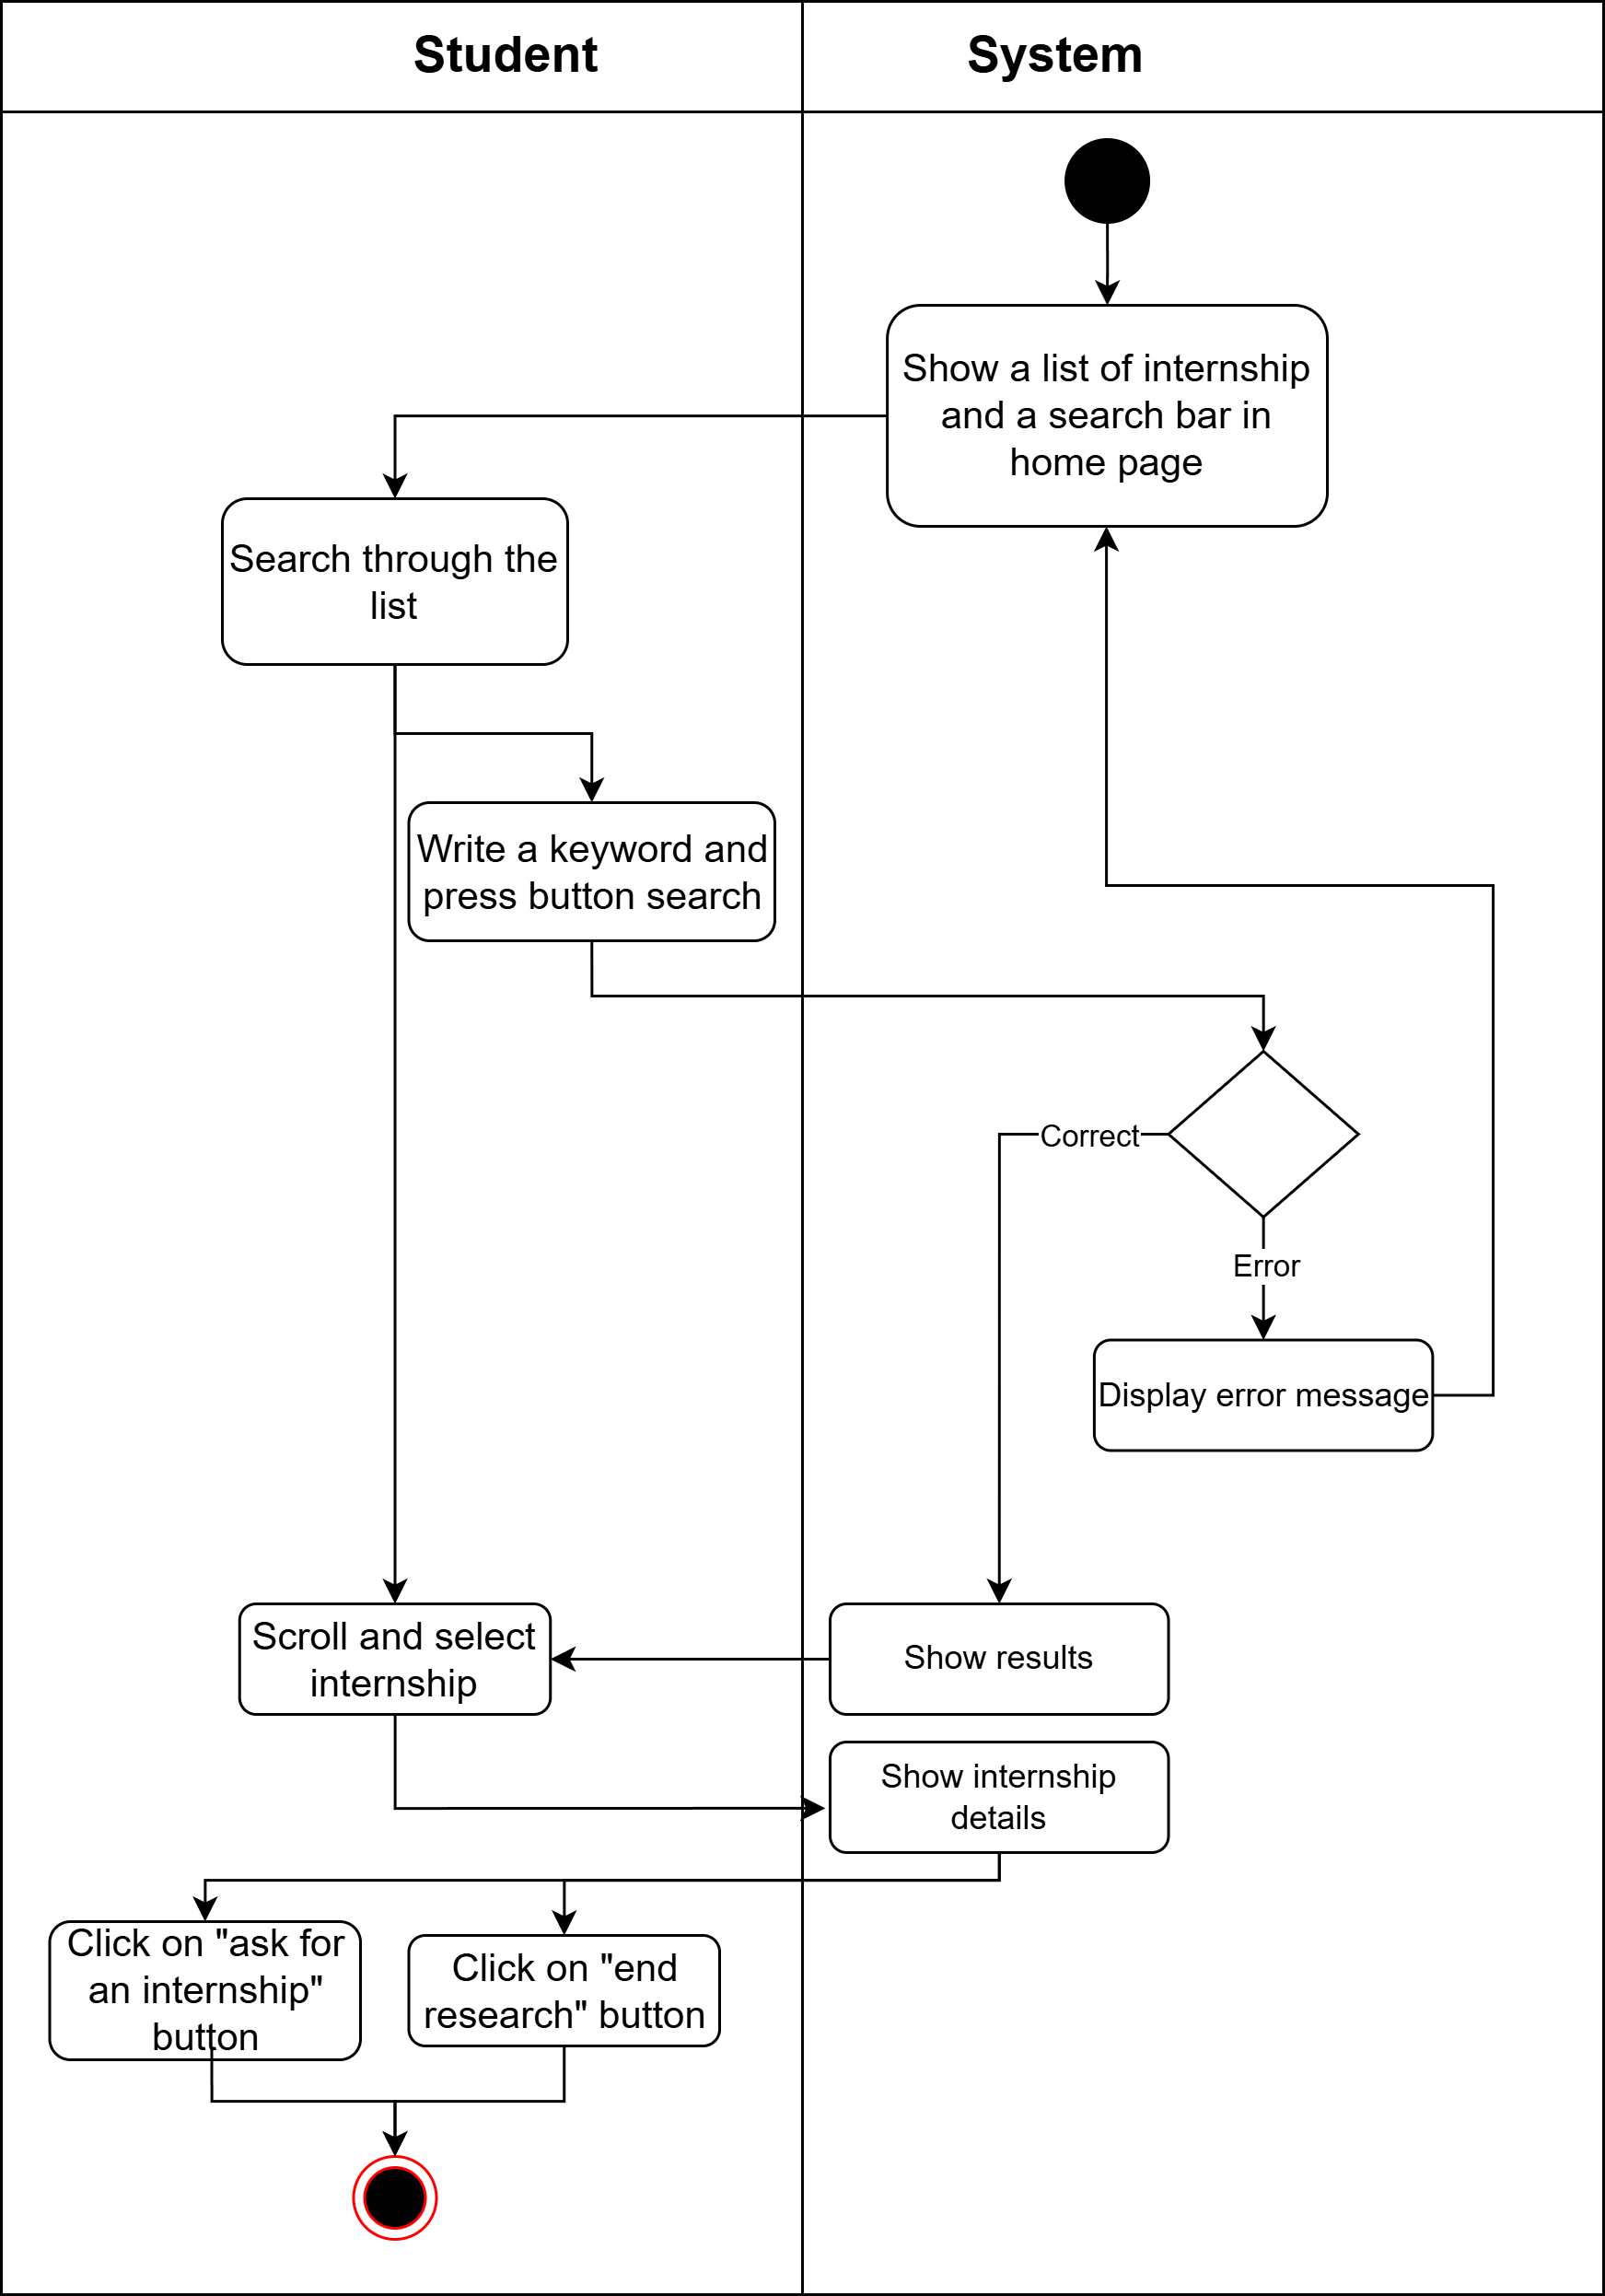
\includegraphics[width=1\linewidth]{Images/UseCasesDiagrams-Student search.png}
    \caption{AD6}
    \label{AD6}
\end{figure}

%uc7
\begin{table}[H]
\renewcommand\arraystretch{1.25}
    \centering
    \begin{tabular}{|l|p{12 cm}|}
    \hline
    \textbf{Name} & Student notification\\
    \hline
    \textbf{Actors} & Student\\
    \hline
    \textbf{Entry conditions} & Recommendation system find a match.\\
    \hline
    \textbf{Events flow} & The notification appears on the main page of the student.\\  
    \hline
    \textbf{Exit conditions} & 
    \begin{enumerate}[label=(\alph*)]
        \item The student decides to accept the internship.
        \item The student decides to reject the internship.
    \end{enumerate}\\
    \hline
    \end{tabular}
    \caption{UC7}
    \label{UC7}
\end{table}

%uc8
\begin{table}[H]
\renewcommand\arraystretch{1.25}
    \centering
    \begin{tabular}{|l|p{12 cm}|}
    \hline
    \textbf{Name} & Company notification\\
    \hline
    \textbf{Actors} & Company\\
    \hline
    \textbf{Entry conditions} & 
    \begin{enumerate}[label=(\alph*)]
        \item A student click the button "Ask for an internship".
        \item Recommendation system find a match.
    \end{enumerate}\\
    \hline
    \textbf{Events flow} & The notification appears on the main page of the company.\\  
    \hline
    \textbf{Exit conditions} & 
    \begin{enumerate}[label=(\alph*)]
        \item The company decides to accept the internship.
        \item The company decides to reject the internship.
    \end{enumerate}\\
    \hline
    \end{tabular}
    \caption{UC8}
    \label{UC8}
\end{table}

%uc9
\begin{table}[H]
\renewcommand\arraystretch{1.25}
    \centering
    \begin{tabular}{|l|p{12 cm}|}
    \hline
    \textbf{Name} & User schedule the interview\\
    \hline
    \textbf{Actors} & Student and company\\
    \hline
    \textbf{Entry conditions} & 
    \begin{enumerate}[label=(\alph*)]
        \item Company accepts the request of the student.
        \item Student and company accept the notification of the recommendation system.
    \end{enumerate}\\
    \hline
    \textbf{Events flow} &
    \begin{enumerate}
        \item User clicks on accepted internship.
        \item User clicks on the calendar icon.
        \item The system shows the calendar.
        \item User the user indicates which days he has free.
    \end{enumerate}\\  
    \hline
    \textbf{Exit conditions} & 
    \begin{enumerate}[label=(\alph*)]
        \item User click the button "save".
        \item User click out the calendar.
    \end{enumerate}\\
    \hline
    \textbf{Exception} & User click the button "save" without indicate the free days\\
    \hline
    \end{tabular}
    \caption{UC9}
    \label{UC9}
\end{table}

%uc11
\begin{table}[H]
\renewcommand\arraystretch{1.25}
    \centering
    \begin{tabular}{|l|p{12 cm}|}
    \hline
    \textbf{Name} & User leave a feedback\\
    \hline
    \textbf{Actors} & Student and company\\
    \hline
    \textbf{Entry conditions} & The internship is over\\
    \hline
    \textbf{Events flow} &
    \begin{enumerate}
        \item User clicks on  finished internship.
        \item The system shows a box where you can write it.
        \item User write the feedback.
    \end{enumerate}\\  
    \hline
    \textbf{Exit conditions} & User click the button "save"\\
    \hline
    \end{tabular}
    \caption{UC11}
    \label{UC11}
\end{table}

%uc12
\begin{table}[H]
\renewcommand\arraystretch{1.25}
    \centering
    \begin{tabular}{|l|p{12 cm}|}
    \hline
    \textbf{Name} & Zoom call \\
    \hline
    \textbf{Actors} & Student and company\\
    \hline
    \textbf{Entry conditions} & S\&C finds a free slot for both of them\\
    \hline
    \textbf{Events flow} &
    \begin{enumerate}
        \item The system communicates with Zoom to create a link for the video-call.
        \item Zoom successfully creates the link.
        \item Zoom sends the link to the system that saves it in the database.
        \item The system show the link on the users page.
    \end{enumerate}\\  
    \hline
    \textbf{Exit conditions} & On the day the internship starts the link is deleted\\
    \hline
    \end{tabular}
    \caption{UC12}
    \label{UC12}
\end{table}

\subsubsection{Requirements}

\begin{table}[H]
\renewcommand\arraystretch{1.5}
    \centering
    \begin{tabular}{ll}
    \hline
    \textbf{R1} & The S\&C platform allows users to register.\\
    \hline
    \textbf{R2} & The S\&C platform allows users to register filling mandatory fields.\\
    \hline
    \textbf{R3} & The S\&C platform allows users to login using their credential.\\
    \hline
    \textbf{R4} & The S\&C platform allows users to manage their data and modify them.\\
    \hline
    \textbf{R5} & The S\&C platform allows companies to insert an internship.\\
    \hline
    \textbf{R6} & The S\&C platform allows company to modify their internships data.\\
    \hline
    \textbf{R7} & The S\&C platform should provide the "search internship" functionality to students.\\
    \hline
    \textbf{R8} & The S\&C platform should notify users when a match is found.\\
    \hline
    \textbf{R9} & The S\&C platform should notify companies when a match is found.\\
    \hline
    \textbf{R10} & The S\&C platform should notify companies when a student request to be contacted.\\
    \hline
    \textbf{R11} & The S\&C platform should allows users to accept or not the match made by the platform.\\
    \hline
    \textbf{R12} & The S\&C platform should send to the students a form related to the chosen internship\\
    \hline
    \textbf{R13} & The user should fill the mandatory form by the deadline\\
    \hline
    \textbf{R14} & The S\&C platform check that the form has been compiled by the deadline\\
    \hline
    \textbf{R15} & The S\&C platform allows user to insert their free slots\\
    \hline
    \textbf{R16} & The S\&C platform should provide a match for a free slot between the users schedules\\
    \hline
    \textbf{R17} & \begin{tabular}[c]{@{}l@{}}The S\&C platform should be able to request zoom to create a call room\\ and receive back the corresponding link.\end{tabular}\\
    \hline
    \textbf{R18} & The S\&C platform should allows users to leave feedback. 
    \end{tabular}
    \caption{Requirements}
    \label{Requirements}
\end{table}

\subsubsection{Mapping on requirements}

\begin{table}[H]
\renewcommand\arraystretch{1.5}
    \centering
    \begin{tabular}{p{10cm}ll}
    \rowcolor{BurntOrange}
        \textbf{Goal}&  \textbf{Requirements}& \textbf{Assumptions}\\
    \hline
    \textbf{[G1]:}All unregistered students and Companies must be able to subscribe and login to the S\&C platform. & R1,R2,R3 & A1,A2,A4,A6\\
    \hline
    \textbf{[G2]:} Companies must be able to create internship offers.& R5, R6 & \\
    \hline
    \textbf{[G3]:} Students must be able to complete their CV and preferences.& R4 & \\
    \hline
    \textbf{[G4]:} Students must be able to search for an internship.& R7 & \\
    \hline
    \textbf{[G5]:} Student and Company are informed when there is a match between them.
    & R8,R9 & \\
    \hline
    \textbf{[G6]:} Monitoring of the execution of the internships.& & \\
    \hline
    \textbf{[G7]:} Statistics collection.& & \\
    \hline
    \textbf{[G8]:} Feedbacks collection.& & \\
    \hline
    \textbf{[G9]:} Companies rank based on Feedback.& & \\
    \hline
    \end{tabular}
    \caption{Mapping on requirements}
    \label{Mapping on requirements}
\end{table}

\subsection{Performance Requirements}
The main performance indicator for this application should be scalability because a large number of users is expected.

\subsection{Design Constraint}
\subsubsection{Standard Compliance}
\begin{itemize}
    \item The platform includes the full adherence to \textbf{GDPR}, which stands as one of the most significant and internationally recognized standards for the protection of personal data and the ensuring of user privacy. The system is committed to handling user data in \textbf{GDPR} compliant ways, ensuring transparency in data collection and processing, and adopting appropriate security measures to protect such data. 
    \item To obtain data correctness and protection even at the communication level, the platform should adopt the use of \textbf{TCP/IP} together with the application of the \textbf{TLS} security protocol. 
    \item The purpose of \textbf{S\&C} is to gather students and companies from all over the world. So, it is very important to use a time standard, such as UTC, to achieve the synchronization of all the users, the correct unfolding of Battles, and the handling of deadlines.
\end{itemize}

\subsubsection{Easy to use}
The application should be very user-friendly to allow the vast majority of people to use it.

\subsubsection{Hardware limitations}
In order to enable an effective use of the platform for as many users as possible, the platform should not require high-level hardware and should work on almost all types of machine. 

\subsubsection{Any other constraint}
S\&C platform is intended to welcome students from all over the world. So, it should be necessarily designed completely in English, allowing every student to understand its pages, interfaces, commands, etc. 

\subsection{Software system attributes}
\subsubsection{Reliability}
The system should prevent downtime, even when the system is stressed with a great number of simultaneous requests, to let users always start and end research and to prevent problems in the selection process.

\subsubsection{Availability}
The system must be available as much as possible to allow the user to benefit from the services when they need them. The system should be available with a minimum value of 99\% of time. Who will be more affected by lack of availability are users. In this case, students may not be able to search the internship list and cannot participate in the selection process.

\subsubsection{Modularity}
The system must be designed in a modular way, both for the client-side and for the server-side. The two kinds of actors will have different interfaces that permit the execution of different functionalities. From the server side, traffic is distributed among several servers and managed through a load balancer server. This solution will also allow the user to use the application during the downtime period needed to maintain the server.

\subsubsection{Maintainability}
It is very important to ensure that the source code of the system can be easily understood, modified, and improved over time. To achieve this goal, the code should be clear and well documented, making it easy for developers to understand and facilitating maintenance.

\subsubsection{Security}
To match the \textbf{GDPR} compliance, the platform should achieve protection of personal data through an authentication system that involves unique usernames and strong passwords.\\ 
There are some aspects of the platform that are private (updating PDF, inserting internships), i.e. they are reserved only for a specific group of users. For this purpose, the platform should provide a keyword-based protection system, capable of generating and managing unique keywords: users are asked to submit the correct keyword to access private contexts. 

\subsubsection{Portability}
Given S\&C's scale and reach, it is crucial to ensure its compatibility with a wide range of operating systems, including Windows, MacOS, and Linux, for an effortless deployment. 

\clearpage
{\color{Blue}{\section{Formal Analysis Using Alloy}}}
\label{sect:alloy}
Organize this section according to the rules defined in the project description. 


\clearpage
{\color{Blue}{\section{Effort Spent}}}
\label{sect:effort}
Provide here information about how much effort each group member spent in working at this document. We would appreciate details here.


\clearpage
\addcontentsline{toc}{section}{References}
\bibliographystyle{plain}
\bibliography{main}

\end{document}

% Sample content




